\documentclass[twoside]{book}

% Packages required by doxygen
\usepackage{fixltx2e}
\usepackage{calc}
\usepackage{doxygen}
\usepackage[export]{adjustbox} % also loads graphicx
\usepackage{graphicx}
\usepackage[utf8]{inputenc}
\usepackage{makeidx}
\usepackage{multicol}
\usepackage{multirow}
\PassOptionsToPackage{warn}{textcomp}
\usepackage{textcomp}
\usepackage[nointegrals]{wasysym}
\usepackage[table]{xcolor}

% Font selection
\usepackage[T1]{fontenc}
\usepackage[scaled=.90]{helvet}
\usepackage{courier}
\usepackage{amssymb}
\usepackage{sectsty}
\renewcommand{\familydefault}{\sfdefault}
\allsectionsfont{%
  \fontseries{bc}\selectfont%
  \color{darkgray}%
}
\renewcommand{\DoxyLabelFont}{%
  \fontseries{bc}\selectfont%
  \color{darkgray}%
}
\newcommand{\+}{\discretionary{\mbox{\scriptsize$\hookleftarrow$}}{}{}}

% Page & text layout
\usepackage{geometry}
\geometry{%
  a4paper,%
  top=2.5cm,%
  bottom=2.5cm,%
  left=2.5cm,%
  right=2.5cm%
}
\tolerance=750
\hfuzz=15pt
\hbadness=750
\setlength{\emergencystretch}{15pt}
\setlength{\parindent}{0cm}
\setlength{\parskip}{3ex plus 2ex minus 2ex}
\makeatletter
\renewcommand{\paragraph}{%
  \@startsection{paragraph}{4}{0ex}{-1.0ex}{1.0ex}{%
    \normalfont\normalsize\bfseries\SS@parafont%
  }%
}
\renewcommand{\subparagraph}{%
  \@startsection{subparagraph}{5}{0ex}{-1.0ex}{1.0ex}{%
    \normalfont\normalsize\bfseries\SS@subparafont%
  }%
}
\makeatother

% Headers & footers
\usepackage{fancyhdr}
\pagestyle{fancyplain}
\fancyhead[LE]{\fancyplain{}{\bfseries\thepage}}
\fancyhead[CE]{\fancyplain{}{}}
\fancyhead[RE]{\fancyplain{}{\bfseries\leftmark}}
\fancyhead[LO]{\fancyplain{}{\bfseries\rightmark}}
\fancyhead[CO]{\fancyplain{}{}}
\fancyhead[RO]{\fancyplain{}{\bfseries\thepage}}
\fancyfoot[LE]{\fancyplain{}{}}
\fancyfoot[CE]{\fancyplain{}{}}
\fancyfoot[RE]{\fancyplain{}{\bfseries\scriptsize Generated by Doxygen }}
\fancyfoot[LO]{\fancyplain{}{\bfseries\scriptsize Generated by Doxygen }}
\fancyfoot[CO]{\fancyplain{}{}}
\fancyfoot[RO]{\fancyplain{}{}}
\renewcommand{\footrulewidth}{0.4pt}
\renewcommand{\chaptermark}[1]{%
  \markboth{#1}{}%
}
\renewcommand{\sectionmark}[1]{%
  \markright{\thesection\ #1}%
}

% Indices & bibliography
\usepackage{natbib}
\usepackage[titles]{tocloft}
\setcounter{tocdepth}{3}
\setcounter{secnumdepth}{5}
\makeindex

% Hyperlinks (required, but should be loaded last)
\usepackage{ifpdf}
\ifpdf
  \usepackage[pdftex,pagebackref=true]{hyperref}
\else
  \usepackage[ps2pdf,pagebackref=true]{hyperref}
\fi
\hypersetup{%
  colorlinks=true,%
  linkcolor=blue,%
  citecolor=blue,%
  unicode%
}

% Custom commands
\newcommand{\clearemptydoublepage}{%
  \newpage{\pagestyle{empty}\cleardoublepage}%
}

\usepackage{caption}
\captionsetup{labelsep=space,justification=centering,font={bf},singlelinecheck=off,skip=4pt,position=top}

%===== C O N T E N T S =====

\begin{document}

% Titlepage & ToC
\hypersetup{pageanchor=false,
             bookmarksnumbered=true,
             pdfencoding=unicode
            }
\pagenumbering{alph}
\begin{titlepage}
\vspace*{7cm}
\begin{center}%
{\Large My Project }\\
\vspace*{1cm}
{\large Generated by Doxygen 1.8.13}\\
\end{center}
\end{titlepage}
\clearemptydoublepage
\pagenumbering{roman}
\tableofcontents
\clearemptydoublepage
\pagenumbering{arabic}
\hypersetup{pageanchor=true}

%--- Begin generated contents ---
\chapter{Hierarchical Index}
\section{Class Hierarchy}
This inheritance list is sorted roughly, but not completely, alphabetically\+:\begin{DoxyCompactList}
\item \contentsline{section}{C\+Aquarium}{\pageref{class_c_aquarium}}{}
\item C\+Dialog\+Ex\begin{DoxyCompactList}
\item \contentsline{section}{C\+About\+Dlg}{\pageref{class_c_about_dlg}}{}
\end{DoxyCompactList}
\item C\+Frame\+Wnd\begin{DoxyCompactList}
\item \contentsline{section}{C\+Main\+Frame}{\pageref{class_c_main_frame}}{}
\end{DoxyCompactList}
\item \contentsline{section}{C\+Item}{\pageref{class_c_item}}{}
\begin{DoxyCompactList}
\item \contentsline{section}{C\+Fish\+Beta}{\pageref{class_c_fish_beta}}{}
\item \contentsline{section}{C\+Fish\+Carp}{\pageref{class_c_fish_carp}}{}
\item \contentsline{section}{C\+Fish\+Magikarp}{\pageref{class_c_fish_magikarp}}{}
\item \contentsline{section}{C\+Fish\+Nemo}{\pageref{class_c_fish_nemo}}{}
\end{DoxyCompactList}
\item C\+Win\+App\begin{DoxyCompactList}
\item \contentsline{section}{C\+Step2\+App}{\pageref{class_c_step2_app}}{}
\end{DoxyCompactList}
\item C\+Wnd\begin{DoxyCompactList}
\item \contentsline{section}{C\+Child\+View}{\pageref{class_c_child_view}}{}
\end{DoxyCompactList}
\end{DoxyCompactList}

\chapter{Class Index}
\section{Class List}
Here are the classes, structs, unions and interfaces with brief descriptions\+:\begin{DoxyCompactList}
\item\contentsline{section}{\hyperlink{class_c_about_dlg}{C\+About\+Dlg} }{\pageref{class_c_about_dlg}}{}
\item\contentsline{section}{\hyperlink{class_c_aquarium}{C\+Aquarium} }{\pageref{class_c_aquarium}}{}
\item\contentsline{section}{\hyperlink{class_c_child_view}{C\+Child\+View} }{\pageref{class_c_child_view}}{}
\item\contentsline{section}{\hyperlink{class_c_fish_beta}{C\+Fish\+Beta} }{\pageref{class_c_fish_beta}}{}
\item\contentsline{section}{\hyperlink{class_c_fish_carp}{C\+Fish\+Carp} }{\pageref{class_c_fish_carp}}{}
\item\contentsline{section}{\hyperlink{class_c_fish_magikarp}{C\+Fish\+Magikarp} }{\pageref{class_c_fish_magikarp}}{}
\item\contentsline{section}{\hyperlink{class_c_fish_nemo}{C\+Fish\+Nemo} }{\pageref{class_c_fish_nemo}}{}
\item\contentsline{section}{\hyperlink{class_c_item}{C\+Item} }{\pageref{class_c_item}}{}
\item\contentsline{section}{\hyperlink{class_c_main_frame}{C\+Main\+Frame} }{\pageref{class_c_main_frame}}{}
\item\contentsline{section}{\hyperlink{class_c_step2_app}{C\+Step2\+App} }{\pageref{class_c_step2_app}}{}
\end{DoxyCompactList}

\chapter{File Index}
\section{File List}
Here is a list of all documented files with brief descriptions\+:\begin{DoxyCompactList}
\item\contentsline{section}{\hyperlink{_aquarium_8cpp}{Aquarium.\+cpp} }{\pageref{_aquarium_8cpp}}{}
\item\contentsline{section}{\hyperlink{_aquarium_8h}{Aquarium.\+h} }{\pageref{_aquarium_8h}}{}
\item\contentsline{section}{\hyperlink{_child_view_8cpp}{Child\+View.\+cpp} }{\pageref{_child_view_8cpp}}{}
\item\contentsline{section}{\hyperlink{_child_view_8h}{Child\+View.\+h} }{\pageref{_child_view_8h}}{}
\item\contentsline{section}{\hyperlink{_double_buffer_d_c_8h}{Double\+Buffer\+D\+C.\+h} \\*Custom device context that supports double buffering }{\pageref{_double_buffer_d_c_8h}}{}
\item\contentsline{section}{\hyperlink{_fish_beta_8cpp}{Fish\+Beta.\+cpp} }{\pageref{_fish_beta_8cpp}}{}
\item\contentsline{section}{\hyperlink{_fish_beta_8h}{Fish\+Beta.\+h} }{\pageref{_fish_beta_8h}}{}
\item\contentsline{section}{\hyperlink{_fish_carp_8cpp}{Fish\+Carp.\+cpp} }{\pageref{_fish_carp_8cpp}}{}
\item\contentsline{section}{\hyperlink{_fish_carp_8h}{Fish\+Carp.\+h} }{\pageref{_fish_carp_8h}}{}
\item\contentsline{section}{\hyperlink{_fish_magikarp_8cpp}{Fish\+Magikarp.\+cpp} }{\pageref{_fish_magikarp_8cpp}}{}
\item\contentsline{section}{\hyperlink{_fish_magikarp_8h}{Fish\+Magikarp.\+h} }{\pageref{_fish_magikarp_8h}}{}
\item\contentsline{section}{\hyperlink{_fish_nemo_8cpp}{Fish\+Nemo.\+cpp} }{\pageref{_fish_nemo_8cpp}}{}
\item\contentsline{section}{\hyperlink{_fish_nemo_8h}{Fish\+Nemo.\+h} }{\pageref{_fish_nemo_8h}}{}
\item\contentsline{section}{\hyperlink{_item_8cpp}{Item.\+cpp} }{\pageref{_item_8cpp}}{}
\item\contentsline{section}{\hyperlink{_item_8h}{Item.\+h} }{\pageref{_item_8h}}{}
\item\contentsline{section}{{\bfseries Main\+Frm.\+h} }{\pageref{_main_frm_8h}}{}
\item\contentsline{section}{{\bfseries resource.\+h} }{\pageref{resource_8h}}{}
\item\contentsline{section}{{\bfseries stdafx.\+h} }{\pageref{stdafx_8h}}{}
\item\contentsline{section}{{\bfseries Step2.\+h} }{\pageref{_step2_8h}}{}
\item\contentsline{section}{{\bfseries targetver.\+h} }{\pageref{targetver_8h}}{}
\end{DoxyCompactList}

\chapter{Class Documentation}
\hypertarget{class_c_about_dlg}{}\section{C\+About\+Dlg Class Reference}
\label{class_c_about_dlg}\index{C\+About\+Dlg@{C\+About\+Dlg}}
Inheritance diagram for C\+About\+Dlg\+:\begin{figure}[H]
\begin{center}
\leavevmode
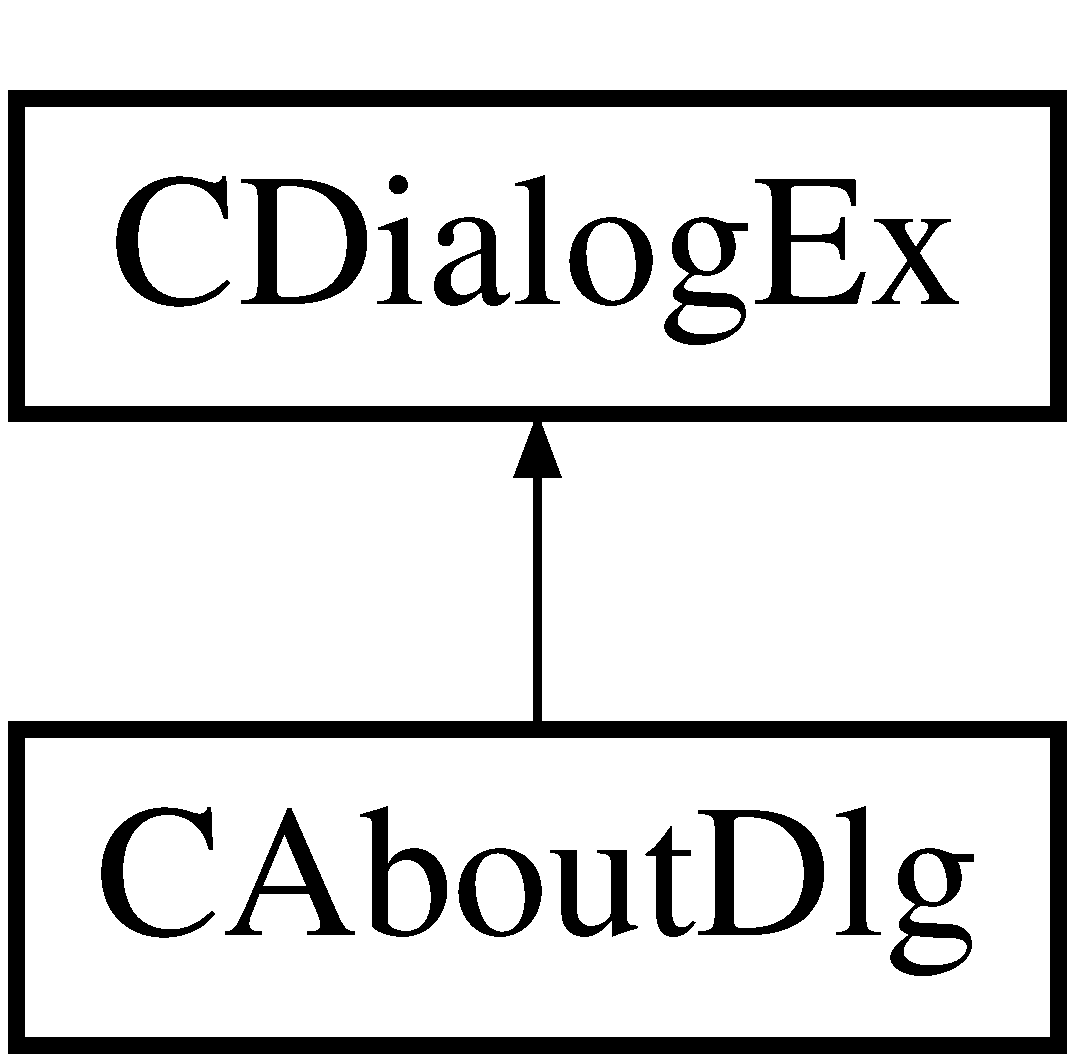
\includegraphics[height=2.000000cm]{class_c_about_dlg}
\end{center}
\end{figure}
\subsection*{Protected Member Functions}
\begin{DoxyCompactItemize}
\item 
\mbox{\Hypertarget{class_c_about_dlg_ab83db7484fec957282d7d5a21aed4df4}\label{class_c_about_dlg_ab83db7484fec957282d7d5a21aed4df4}} 
virtual void {\bfseries Do\+Data\+Exchange} (C\+Data\+Exchange $\ast$p\+DX)
\end{DoxyCompactItemize}


The documentation for this class was generated from the following file\+:\begin{DoxyCompactItemize}
\item 
Step2.\+cpp\end{DoxyCompactItemize}

\hypertarget{class_c_aquarium}{}\section{C\+Aquarium Class Reference}
\label{class_c_aquarium}\index{C\+Aquarium@{C\+Aquarium}}


{\ttfamily \#include $<$Aquarium.\+h$>$}

\subsection*{Public Member Functions}
\begin{DoxyCompactItemize}
\item 
\hyperlink{class_c_aquarium_ab6ba8b1abd87437ff66748e82173a5a8}{C\+Aquarium} ()
\item 
virtual \hyperlink{class_c_aquarium_ab1baf78dc047af2b8cab8982e1446875}{$\sim$\+C\+Aquarium} ()
\item 
void \hyperlink{class_c_aquarium_a20b4899158d1ba4bc41217630d47e180}{On\+Draw} (Gdiplus\+::\+Graphics $\ast$graphics)
\item 
void \hyperlink{class_c_aquarium_a85063d05c147cf80f54182016fe12d64}{Add} (std\+::shared\+\_\+ptr$<$ \hyperlink{class_c_item}{C\+Item} $>$ item)
\item 
std\+::shared\+\_\+ptr$<$ \hyperlink{class_c_item}{C\+Item} $>$ \hyperlink{class_c_aquarium_a7129486467e76938fbc049723f9187f3}{Hit\+Test} (int x, int y)
\item 
void \hyperlink{class_c_aquarium_a44230dbff0c91121b55baae49e6fbb5e}{Move\+To\+Front} (std\+::shared\+\_\+ptr$<$ \hyperlink{class_c_item}{C\+Item} $>$ item)
\item 
virtual void \hyperlink{class_c_aquarium_ae159ee63d91f3a4b37644640fa67fdd8}{Kill\+Fish} (std\+::shared\+\_\+ptr$<$ \hyperlink{class_c_item}{C\+Item} $>$ item)
\item 
void \hyperlink{class_c_aquarium_a600f0ffe730776b9d5539511a4b191b9}{Delete\+Item} (std\+::shared\+\_\+ptr$<$ \hyperlink{class_c_item}{C\+Item} $>$ item)
\end{DoxyCompactItemize}


\subsection{Detailed Description}
Represents an aquarium 

\subsection{Constructor \& Destructor Documentation}
\mbox{\Hypertarget{class_c_aquarium_ab6ba8b1abd87437ff66748e82173a5a8}\label{class_c_aquarium_ab6ba8b1abd87437ff66748e82173a5a8}} 
\index{C\+Aquarium@{C\+Aquarium}!C\+Aquarium@{C\+Aquarium}}
\index{C\+Aquarium@{C\+Aquarium}!C\+Aquarium@{C\+Aquarium}}
\subsubsection{\texorpdfstring{C\+Aquarium()}{CAquarium()}}
{\footnotesize\ttfamily C\+Aquarium\+::\+C\+Aquarium (\begin{DoxyParamCaption}{ }\end{DoxyParamCaption})}

Constructor \mbox{\Hypertarget{class_c_aquarium_ab1baf78dc047af2b8cab8982e1446875}\label{class_c_aquarium_ab1baf78dc047af2b8cab8982e1446875}} 
\index{C\+Aquarium@{C\+Aquarium}!````~C\+Aquarium@{$\sim$\+C\+Aquarium}}
\index{````~C\+Aquarium@{$\sim$\+C\+Aquarium}!C\+Aquarium@{C\+Aquarium}}
\subsubsection{\texorpdfstring{$\sim$\+C\+Aquarium()}{~CAquarium()}}
{\footnotesize\ttfamily C\+Aquarium\+::$\sim$\+C\+Aquarium (\begin{DoxyParamCaption}{ }\end{DoxyParamCaption})\hspace{0.3cm}{\ttfamily [virtual]}}

Destructor 

\subsection{Member Function Documentation}
\mbox{\Hypertarget{class_c_aquarium_a85063d05c147cf80f54182016fe12d64}\label{class_c_aquarium_a85063d05c147cf80f54182016fe12d64}} 
\index{C\+Aquarium@{C\+Aquarium}!Add@{Add}}
\index{Add@{Add}!C\+Aquarium@{C\+Aquarium}}
\subsubsection{\texorpdfstring{Add()}{Add()}}
{\footnotesize\ttfamily void C\+Aquarium\+::\+Add (\begin{DoxyParamCaption}\item[{std\+::shared\+\_\+ptr$<$ \hyperlink{class_c_item}{C\+Item} $>$}]{item }\end{DoxyParamCaption})}

Add an item to the aquarium 
\begin{DoxyParams}{Parameters}
{\em item} & New item to add \\
\hline
\end{DoxyParams}
\mbox{\Hypertarget{class_c_aquarium_a600f0ffe730776b9d5539511a4b191b9}\label{class_c_aquarium_a600f0ffe730776b9d5539511a4b191b9}} 
\index{C\+Aquarium@{C\+Aquarium}!Delete\+Item@{Delete\+Item}}
\index{Delete\+Item@{Delete\+Item}!C\+Aquarium@{C\+Aquarium}}
\subsubsection{\texorpdfstring{Delete\+Item()}{DeleteItem()}}
{\footnotesize\ttfamily void C\+Aquarium\+::\+Delete\+Item (\begin{DoxyParamCaption}\item[{std\+::shared\+\_\+ptr$<$ \hyperlink{class_c_item}{C\+Item} $>$}]{item }\end{DoxyParamCaption})}

Deletes item from m\+Items 
\begin{DoxyParams}{Parameters}
{\em item} & Item to delete \\
\hline
\end{DoxyParams}
\mbox{\Hypertarget{class_c_aquarium_a7129486467e76938fbc049723f9187f3}\label{class_c_aquarium_a7129486467e76938fbc049723f9187f3}} 
\index{C\+Aquarium@{C\+Aquarium}!Hit\+Test@{Hit\+Test}}
\index{Hit\+Test@{Hit\+Test}!C\+Aquarium@{C\+Aquarium}}
\subsubsection{\texorpdfstring{Hit\+Test()}{HitTest()}}
{\footnotesize\ttfamily std\+::shared\+\_\+ptr$<$ \hyperlink{class_c_item}{C\+Item} $>$ C\+Aquarium\+::\+Hit\+Test (\begin{DoxyParamCaption}\item[{int}]{x,  }\item[{int}]{y }\end{DoxyParamCaption})}

Test an x,y click location to see if it clicked on some item in the aquarium. 
\begin{DoxyParams}{Parameters}
{\em x} & X location \\
\hline
{\em y} & Y location \\
\hline
\end{DoxyParams}
\begin{DoxyReturn}{Returns}
Pointer to item we clicked on or nullptr if none. 
\end{DoxyReturn}
\mbox{\Hypertarget{class_c_aquarium_ae159ee63d91f3a4b37644640fa67fdd8}\label{class_c_aquarium_ae159ee63d91f3a4b37644640fa67fdd8}} 
\index{C\+Aquarium@{C\+Aquarium}!Kill\+Fish@{Kill\+Fish}}
\index{Kill\+Fish@{Kill\+Fish}!C\+Aquarium@{C\+Aquarium}}
\subsubsection{\texorpdfstring{Kill\+Fish()}{KillFish()}}
{\footnotesize\ttfamily void C\+Aquarium\+::\+Kill\+Fish (\begin{DoxyParamCaption}\item[{std\+::shared\+\_\+ptr$<$ \hyperlink{class_c_item}{C\+Item} $>$}]{item }\end{DoxyParamCaption})\hspace{0.3cm}{\ttfamily [virtual]}}

When item is a predator and dragged in front of another item, kills the other item 
\begin{DoxyParams}{Parameters}
{\em item} & Possible predator \\
\hline
\end{DoxyParams}
\mbox{\Hypertarget{class_c_aquarium_a44230dbff0c91121b55baae49e6fbb5e}\label{class_c_aquarium_a44230dbff0c91121b55baae49e6fbb5e}} 
\index{C\+Aquarium@{C\+Aquarium}!Move\+To\+Front@{Move\+To\+Front}}
\index{Move\+To\+Front@{Move\+To\+Front}!C\+Aquarium@{C\+Aquarium}}
\subsubsection{\texorpdfstring{Move\+To\+Front()}{MoveToFront()}}
{\footnotesize\ttfamily void C\+Aquarium\+::\+Move\+To\+Front (\begin{DoxyParamCaption}\item[{std\+::shared\+\_\+ptr$<$ \hyperlink{class_c_item}{C\+Item} $>$}]{item }\end{DoxyParamCaption})}

Move an item to the front of screen 
\begin{DoxyParams}{Parameters}
{\em item} & Item to bring to front \\
\hline
\end{DoxyParams}
\mbox{\Hypertarget{class_c_aquarium_a20b4899158d1ba4bc41217630d47e180}\label{class_c_aquarium_a20b4899158d1ba4bc41217630d47e180}} 
\index{C\+Aquarium@{C\+Aquarium}!On\+Draw@{On\+Draw}}
\index{On\+Draw@{On\+Draw}!C\+Aquarium@{C\+Aquarium}}
\subsubsection{\texorpdfstring{On\+Draw()}{OnDraw()}}
{\footnotesize\ttfamily void C\+Aquarium\+::\+On\+Draw (\begin{DoxyParamCaption}\item[{Gdiplus\+::\+Graphics $\ast$}]{graphics }\end{DoxyParamCaption})}

Draw the aquarium 
\begin{DoxyParams}{Parameters}
{\em graphics} & The G\+D\+I+ graphics context to draw on \\
\hline
\end{DoxyParams}


The documentation for this class was generated from the following files\+:\begin{DoxyCompactItemize}
\item 
\hyperlink{_aquarium_8h}{Aquarium.\+h}\item 
\hyperlink{_aquarium_8cpp}{Aquarium.\+cpp}\end{DoxyCompactItemize}

\hypertarget{class_c_child_view}{}\section{C\+Child\+View Class Reference}
\label{class_c_child_view}\index{C\+Child\+View@{C\+Child\+View}}


{\ttfamily \#include $<$Child\+View.\+h$>$}

Inheritance diagram for C\+Child\+View\+:\begin{figure}[H]
\begin{center}
\leavevmode
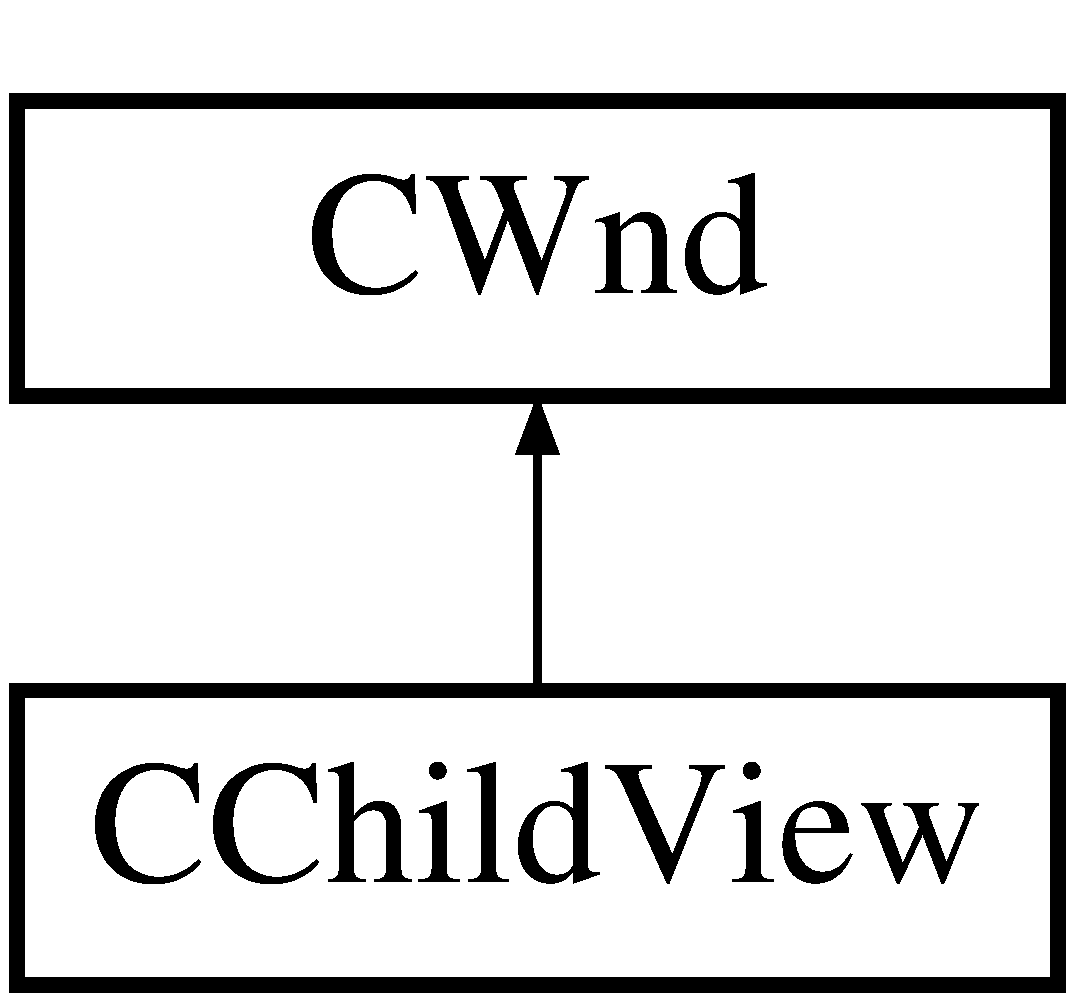
\includegraphics[height=2.000000cm]{class_c_child_view}
\end{center}
\end{figure}
\subsection*{Public Member Functions}
\begin{DoxyCompactItemize}
\item 
\hyperlink{class_c_child_view_aff5af7c162c10755edbe58f260ded6d4}{C\+Child\+View} ()
\begin{DoxyCompactList}\small\item\em Constructor. \end{DoxyCompactList}\item 
virtual \hyperlink{class_c_child_view_a5b033b5e0a130950719a173b86418698}{$\sim$\+C\+Child\+View} ()
\item 
afx\+\_\+msg void \hyperlink{class_c_child_view_af513a57c45ce8b9dcc09dd934e228534}{On\+L\+Button\+Down} (U\+I\+NT n\+Flags, C\+Point point)
\begin{DoxyCompactList}\small\item\em Called when there is a left mouse button press. \end{DoxyCompactList}\item 
afx\+\_\+msg void \hyperlink{class_c_child_view_ae81948a77ebf3744bd0f9449af57ee21}{On\+L\+Button\+Up} (U\+I\+NT n\+Flags, C\+Point point)
\begin{DoxyCompactList}\small\item\em Called when the left mouse button is released. \end{DoxyCompactList}\item 
afx\+\_\+msg void \hyperlink{class_c_child_view_ad3cb2f8d9fa9a6fb06989513dee5a8bc}{On\+Mouse\+Move} (U\+I\+NT n\+Flags, C\+Point point)
\begin{DoxyCompactList}\small\item\em Called when the mouse is moved. \end{DoxyCompactList}\item 
afx\+\_\+msg B\+O\+OL \hyperlink{class_c_child_view_a6060e6d09d522d345dcee5a01d41c1f0}{On\+Erase\+Bkgnd} (C\+DC $\ast$p\+DC)
\begin{DoxyCompactList}\small\item\em Erase the background. \end{DoxyCompactList}\item 
afx\+\_\+msg void \hyperlink{class_c_child_view_a3d54ea142fb2facf2f19fa6772346667}{On\+Add\+Fish\+Beta\+Fish} ()
\begin{DoxyCompactList}\small\item\em Add a beta fish. \end{DoxyCompactList}\item 
afx\+\_\+msg void \hyperlink{class_c_child_view_ae57ff94ee7cff8741c8d5a88c7fbba65}{On\+Add\+Fish\+Magikarp} ()
\begin{DoxyCompactList}\small\item\em Add a magikarp. \end{DoxyCompactList}\item 
afx\+\_\+msg void \hyperlink{class_c_child_view_a425e5b13c9f4bbb54628fc15e5f9cf24}{On\+Add\+Fish\+Nemo} ()
\begin{DoxyCompactList}\small\item\em Add a nemo. \end{DoxyCompactList}\item 
afx\+\_\+msg void \hyperlink{class_c_child_view_a767a63adaaaebeb086861a27fdf36c8c}{On\+Add\+Fish\+Carp} ()
\begin{DoxyCompactList}\small\item\em Add a carp. \end{DoxyCompactList}\end{DoxyCompactItemize}
\subsection*{Public Attributes}
\begin{DoxyCompactItemize}
\item 
\mbox{\Hypertarget{class_c_child_view_a5666495f6927ddc0636738dc02db8c3f}\label{class_c_child_view_a5666495f6927ddc0636738dc02db8c3f}} 
std\+::shared\+\_\+ptr$<$ \hyperlink{class_c_item}{C\+Item} $>$ \hyperlink{class_c_child_view_a5666495f6927ddc0636738dc02db8c3f}{m\+Grabbed\+Item}
\begin{DoxyCompactList}\small\item\em Any item we are currently dragging. \end{DoxyCompactList}\end{DoxyCompactItemize}
\subsection*{Protected Member Functions}
\begin{DoxyCompactItemize}
\item 
\mbox{\Hypertarget{class_c_child_view_a072cbcba60255377ac9d82aed9a14ce8}\label{class_c_child_view_a072cbcba60255377ac9d82aed9a14ce8}} 
virtual B\+O\+OL \hyperlink{class_c_child_view_a072cbcba60255377ac9d82aed9a14ce8}{Pre\+Create\+Window} (C\+R\+E\+A\+T\+E\+S\+T\+R\+U\+CT \&cs)
\begin{DoxyCompactList}\small\item\em This function is called before the window is created. \end{DoxyCompactList}\item 
afx\+\_\+msg void \hyperlink{class_c_child_view_a8ea6d42631a4f9f446923ff864b239ab}{On\+Paint} ()
\begin{DoxyCompactList}\small\item\em This function is called to draw in the window. \end{DoxyCompactList}\end{DoxyCompactItemize}


\subsection{Detailed Description}
The child window our program draws in. 

\subsection{Constructor \& Destructor Documentation}
\mbox{\Hypertarget{class_c_child_view_aff5af7c162c10755edbe58f260ded6d4}\label{class_c_child_view_aff5af7c162c10755edbe58f260ded6d4}} 
\index{C\+Child\+View@{C\+Child\+View}!C\+Child\+View@{C\+Child\+View}}
\index{C\+Child\+View@{C\+Child\+View}!C\+Child\+View@{C\+Child\+View}}
\subsubsection{\texorpdfstring{C\+Child\+View()}{CChildView()}}
{\footnotesize\ttfamily C\+Child\+View\+::\+C\+Child\+View (\begin{DoxyParamCaption}{ }\end{DoxyParamCaption})}



Constructor. 

Constructor \mbox{\Hypertarget{class_c_child_view_a5b033b5e0a130950719a173b86418698}\label{class_c_child_view_a5b033b5e0a130950719a173b86418698}} 
\index{C\+Child\+View@{C\+Child\+View}!````~C\+Child\+View@{$\sim$\+C\+Child\+View}}
\index{````~C\+Child\+View@{$\sim$\+C\+Child\+View}!C\+Child\+View@{C\+Child\+View}}
\subsubsection{\texorpdfstring{$\sim$\+C\+Child\+View()}{~CChildView()}}
{\footnotesize\ttfamily C\+Child\+View\+::$\sim$\+C\+Child\+View (\begin{DoxyParamCaption}{ }\end{DoxyParamCaption})\hspace{0.3cm}{\ttfamily [virtual]}}

Destructor 

\subsection{Member Function Documentation}
\mbox{\Hypertarget{class_c_child_view_a3d54ea142fb2facf2f19fa6772346667}\label{class_c_child_view_a3d54ea142fb2facf2f19fa6772346667}} 
\index{C\+Child\+View@{C\+Child\+View}!On\+Add\+Fish\+Beta\+Fish@{On\+Add\+Fish\+Beta\+Fish}}
\index{On\+Add\+Fish\+Beta\+Fish@{On\+Add\+Fish\+Beta\+Fish}!C\+Child\+View@{C\+Child\+View}}
\subsubsection{\texorpdfstring{On\+Add\+Fish\+Beta\+Fish()}{OnAddFishBetaFish()}}
{\footnotesize\ttfamily void C\+Child\+View\+::\+On\+Add\+Fish\+Beta\+Fish (\begin{DoxyParamCaption}{ }\end{DoxyParamCaption})}



Add a beta fish. 

Adds a beta fish to aquarium \mbox{\Hypertarget{class_c_child_view_a767a63adaaaebeb086861a27fdf36c8c}\label{class_c_child_view_a767a63adaaaebeb086861a27fdf36c8c}} 
\index{C\+Child\+View@{C\+Child\+View}!On\+Add\+Fish\+Carp@{On\+Add\+Fish\+Carp}}
\index{On\+Add\+Fish\+Carp@{On\+Add\+Fish\+Carp}!C\+Child\+View@{C\+Child\+View}}
\subsubsection{\texorpdfstring{On\+Add\+Fish\+Carp()}{OnAddFishCarp()}}
{\footnotesize\ttfamily void C\+Child\+View\+::\+On\+Add\+Fish\+Carp (\begin{DoxyParamCaption}{ }\end{DoxyParamCaption})}



Add a carp. 

Adds a carp to aquarium \mbox{\Hypertarget{class_c_child_view_ae57ff94ee7cff8741c8d5a88c7fbba65}\label{class_c_child_view_ae57ff94ee7cff8741c8d5a88c7fbba65}} 
\index{C\+Child\+View@{C\+Child\+View}!On\+Add\+Fish\+Magikarp@{On\+Add\+Fish\+Magikarp}}
\index{On\+Add\+Fish\+Magikarp@{On\+Add\+Fish\+Magikarp}!C\+Child\+View@{C\+Child\+View}}
\subsubsection{\texorpdfstring{On\+Add\+Fish\+Magikarp()}{OnAddFishMagikarp()}}
{\footnotesize\ttfamily void C\+Child\+View\+::\+On\+Add\+Fish\+Magikarp (\begin{DoxyParamCaption}{ }\end{DoxyParamCaption})}



Add a magikarp. 

Adds a magikarp to aquarium \mbox{\Hypertarget{class_c_child_view_a425e5b13c9f4bbb54628fc15e5f9cf24}\label{class_c_child_view_a425e5b13c9f4bbb54628fc15e5f9cf24}} 
\index{C\+Child\+View@{C\+Child\+View}!On\+Add\+Fish\+Nemo@{On\+Add\+Fish\+Nemo}}
\index{On\+Add\+Fish\+Nemo@{On\+Add\+Fish\+Nemo}!C\+Child\+View@{C\+Child\+View}}
\subsubsection{\texorpdfstring{On\+Add\+Fish\+Nemo()}{OnAddFishNemo()}}
{\footnotesize\ttfamily void C\+Child\+View\+::\+On\+Add\+Fish\+Nemo (\begin{DoxyParamCaption}{ }\end{DoxyParamCaption})}



Add a nemo. 

Adds nemo to aquarium \mbox{\Hypertarget{class_c_child_view_a6060e6d09d522d345dcee5a01d41c1f0}\label{class_c_child_view_a6060e6d09d522d345dcee5a01d41c1f0}} 
\index{C\+Child\+View@{C\+Child\+View}!On\+Erase\+Bkgnd@{On\+Erase\+Bkgnd}}
\index{On\+Erase\+Bkgnd@{On\+Erase\+Bkgnd}!C\+Child\+View@{C\+Child\+View}}
\subsubsection{\texorpdfstring{On\+Erase\+Bkgnd()}{OnEraseBkgnd()}}
{\footnotesize\ttfamily B\+O\+OL C\+Child\+View\+::\+On\+Erase\+Bkgnd (\begin{DoxyParamCaption}\item[{C\+DC $\ast$}]{p\+DC }\end{DoxyParamCaption})}



Erase the background. 

Erase the background

This is disabled to eliminate flicker 
\begin{DoxyParams}{Parameters}
{\em p\+DC} & Device context \\
\hline
\end{DoxyParams}
\begin{DoxyReturn}{Returns}
F\+A\+L\+SE 
\end{DoxyReturn}
\mbox{\Hypertarget{class_c_child_view_af513a57c45ce8b9dcc09dd934e228534}\label{class_c_child_view_af513a57c45ce8b9dcc09dd934e228534}} 
\index{C\+Child\+View@{C\+Child\+View}!On\+L\+Button\+Down@{On\+L\+Button\+Down}}
\index{On\+L\+Button\+Down@{On\+L\+Button\+Down}!C\+Child\+View@{C\+Child\+View}}
\subsubsection{\texorpdfstring{On\+L\+Button\+Down()}{OnLButtonDown()}}
{\footnotesize\ttfamily void C\+Child\+View\+::\+On\+L\+Button\+Down (\begin{DoxyParamCaption}\item[{U\+I\+NT}]{n\+Flags,  }\item[{C\+Point}]{point }\end{DoxyParamCaption})}



Called when there is a left mouse button press. 

Called when there is a left mouse button press 
\begin{DoxyParams}{Parameters}
{\em n\+Flags} & Flags associated with the mouse button press \\
\hline
{\em point} & Where the button was pressed \\
\hline
\end{DoxyParams}
\mbox{\Hypertarget{class_c_child_view_ae81948a77ebf3744bd0f9449af57ee21}\label{class_c_child_view_ae81948a77ebf3744bd0f9449af57ee21}} 
\index{C\+Child\+View@{C\+Child\+View}!On\+L\+Button\+Up@{On\+L\+Button\+Up}}
\index{On\+L\+Button\+Up@{On\+L\+Button\+Up}!C\+Child\+View@{C\+Child\+View}}
\subsubsection{\texorpdfstring{On\+L\+Button\+Up()}{OnLButtonUp()}}
{\footnotesize\ttfamily void C\+Child\+View\+::\+On\+L\+Button\+Up (\begin{DoxyParamCaption}\item[{U\+I\+NT}]{n\+Flags,  }\item[{C\+Point}]{point }\end{DoxyParamCaption})}



Called when the left mouse button is released. 

Called when the left mouse button is released 
\begin{DoxyParams}{Parameters}
{\em n\+Flags} & Flags associated with the mouse button release \\
\hline
{\em point} & Where the button was pressed \\
\hline
\end{DoxyParams}
\mbox{\Hypertarget{class_c_child_view_ad3cb2f8d9fa9a6fb06989513dee5a8bc}\label{class_c_child_view_ad3cb2f8d9fa9a6fb06989513dee5a8bc}} 
\index{C\+Child\+View@{C\+Child\+View}!On\+Mouse\+Move@{On\+Mouse\+Move}}
\index{On\+Mouse\+Move@{On\+Mouse\+Move}!C\+Child\+View@{C\+Child\+View}}
\subsubsection{\texorpdfstring{On\+Mouse\+Move()}{OnMouseMove()}}
{\footnotesize\ttfamily void C\+Child\+View\+::\+On\+Mouse\+Move (\begin{DoxyParamCaption}\item[{U\+I\+NT}]{n\+Flags,  }\item[{C\+Point}]{point }\end{DoxyParamCaption})}



Called when the mouse is moved. 

Called when the mouse is moved 
\begin{DoxyParams}{Parameters}
{\em n\+Flags} & Flags associated with the mouse movement \\
\hline
{\em point} & Where the button was pressed \\
\hline
\end{DoxyParams}
\mbox{\Hypertarget{class_c_child_view_a8ea6d42631a4f9f446923ff864b239ab}\label{class_c_child_view_a8ea6d42631a4f9f446923ff864b239ab}} 
\index{C\+Child\+View@{C\+Child\+View}!On\+Paint@{On\+Paint}}
\index{On\+Paint@{On\+Paint}!C\+Child\+View@{C\+Child\+View}}
\subsubsection{\texorpdfstring{On\+Paint()}{OnPaint()}}
{\footnotesize\ttfamily void C\+Child\+View\+::\+On\+Paint (\begin{DoxyParamCaption}{ }\end{DoxyParamCaption})\hspace{0.3cm}{\ttfamily [protected]}}



This function is called to draw in the window. 

This function is called to draw in the window.

This function is called in response to a drawing message whenever we need to redraw the window on the screen. It is responsible for painting the window. 

The documentation for this class was generated from the following files\+:\begin{DoxyCompactItemize}
\item 
\hyperlink{_child_view_8h}{Child\+View.\+h}\item 
\hyperlink{_child_view_8cpp}{Child\+View.\+cpp}\end{DoxyCompactItemize}

\hypertarget{class_c_fish_beta}{}\section{C\+Fish\+Beta Class Reference}
\label{class_c_fish_beta}\index{C\+Fish\+Beta@{C\+Fish\+Beta}}


{\ttfamily \#include $<$Fish\+Beta.\+h$>$}

Inheritance diagram for C\+Fish\+Beta\+:\begin{figure}[H]
\begin{center}
\leavevmode
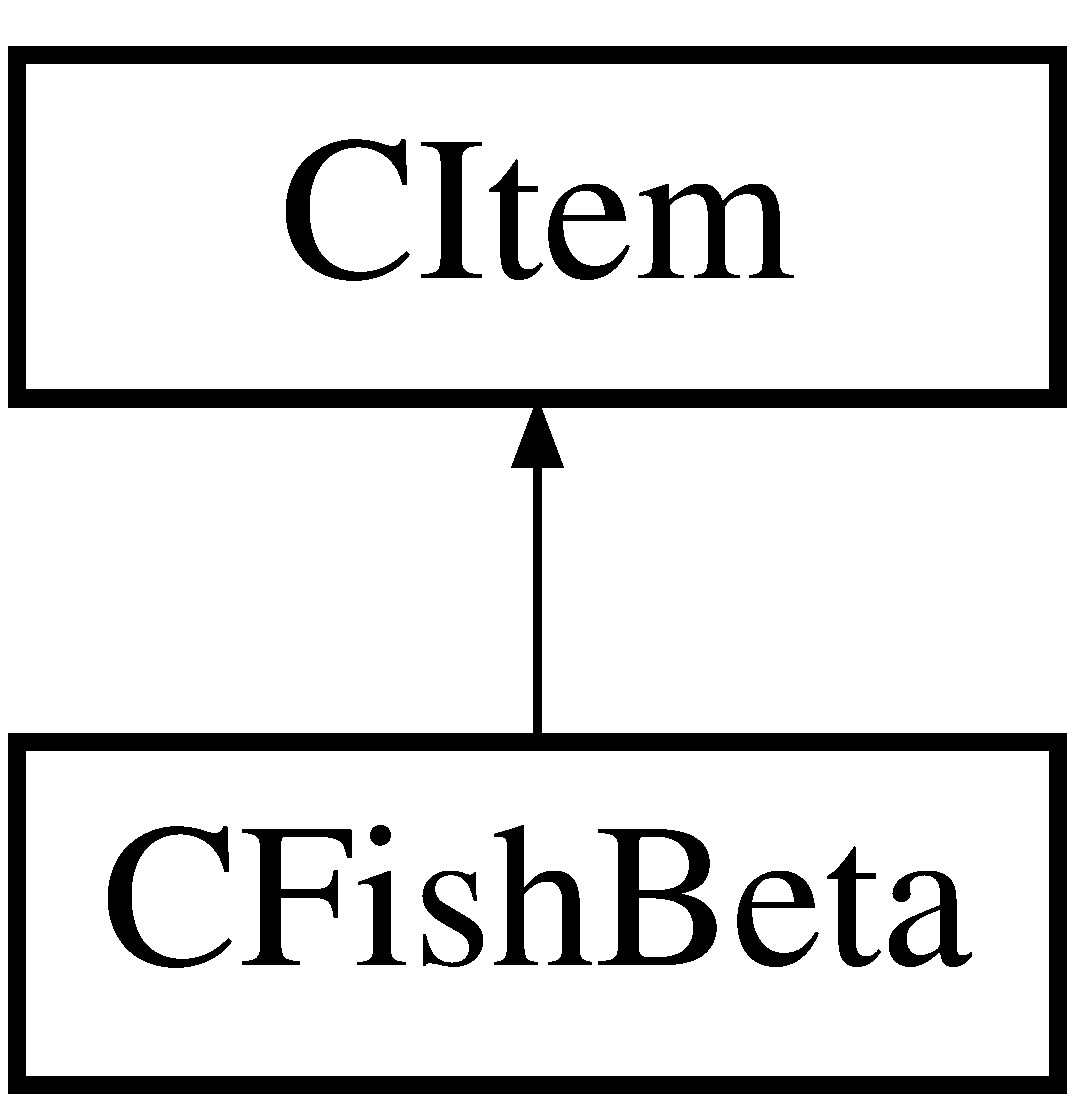
\includegraphics[height=2.000000cm]{class_c_fish_beta}
\end{center}
\end{figure}
\subsection*{Public Member Functions}
\begin{DoxyCompactItemize}
\item 
\hyperlink{class_c_fish_beta_a021073e2e0034271cd7e776b1e3fed29}{C\+Fish\+Beta} (\hyperlink{class_c_aquarium}{C\+Aquarium} $\ast$aquarium)
\begin{DoxyCompactList}\small\item\em Constructor. \end{DoxyCompactList}\item 
\mbox{\Hypertarget{class_c_fish_beta_a4e4d132618735adad44d04c9c40687ca}\label{class_c_fish_beta_a4e4d132618735adad44d04c9c40687ca}} 
\hyperlink{class_c_fish_beta_a4e4d132618735adad44d04c9c40687ca}{C\+Fish\+Beta} ()=delete
\begin{DoxyCompactList}\small\item\em Default constructor (disabled) \end{DoxyCompactList}\item 
\mbox{\Hypertarget{class_c_fish_beta_adbf3559baac135dff393729c51b1ab31}\label{class_c_fish_beta_adbf3559baac135dff393729c51b1ab31}} 
\hyperlink{class_c_fish_beta_adbf3559baac135dff393729c51b1ab31}{C\+Fish\+Beta} (const \hyperlink{class_c_fish_beta}{C\+Fish\+Beta} \&)=delete
\begin{DoxyCompactList}\small\item\em Copy constructor (disabled) \end{DoxyCompactList}\item 
virtual \hyperlink{class_c_fish_beta_abd932894ad25a70f03c79c4f0f00fff4}{$\sim$\+C\+Fish\+Beta} ()
\begin{DoxyCompactList}\small\item\em Destructor. \end{DoxyCompactList}\item 
virtual void \hyperlink{class_c_fish_beta_ae2effbff7b98bb3cd6e1070d61d5366e}{Draw} (Gdiplus\+::\+Graphics $\ast$graphics)
\begin{DoxyCompactList}\small\item\em Draws beta fish. \end{DoxyCompactList}\item 
bool \hyperlink{class_c_fish_beta_a5bdd3d07a57ca1f01a7f2c5c00e0a662}{Hit\+Test} (int x, int y)
\begin{DoxyCompactList}\small\item\em Test to see if we hit this object with a mouse. \end{DoxyCompactList}\end{DoxyCompactItemize}
\subsection*{Additional Inherited Members}


\subsection{Detailed Description}
Implements a Beta fish 

\subsection{Constructor \& Destructor Documentation}
\mbox{\Hypertarget{class_c_fish_beta_a021073e2e0034271cd7e776b1e3fed29}\label{class_c_fish_beta_a021073e2e0034271cd7e776b1e3fed29}} 
\index{C\+Fish\+Beta@{C\+Fish\+Beta}!C\+Fish\+Beta@{C\+Fish\+Beta}}
\index{C\+Fish\+Beta@{C\+Fish\+Beta}!C\+Fish\+Beta@{C\+Fish\+Beta}}
\subsubsection{\texorpdfstring{C\+Fish\+Beta()}{CFishBeta()}}
{\footnotesize\ttfamily C\+Fish\+Beta\+::\+C\+Fish\+Beta (\begin{DoxyParamCaption}\item[{\hyperlink{class_c_aquarium}{C\+Aquarium} $\ast$}]{aquarium }\end{DoxyParamCaption})}



Constructor. 

Constructor 
\begin{DoxyParams}{Parameters}
{\em aquarium} & The aquarium this is a member of \\
\hline
\end{DoxyParams}
\mbox{\Hypertarget{class_c_fish_beta_abd932894ad25a70f03c79c4f0f00fff4}\label{class_c_fish_beta_abd932894ad25a70f03c79c4f0f00fff4}} 
\index{C\+Fish\+Beta@{C\+Fish\+Beta}!````~C\+Fish\+Beta@{$\sim$\+C\+Fish\+Beta}}
\index{````~C\+Fish\+Beta@{$\sim$\+C\+Fish\+Beta}!C\+Fish\+Beta@{C\+Fish\+Beta}}
\subsubsection{\texorpdfstring{$\sim$\+C\+Fish\+Beta()}{~CFishBeta()}}
{\footnotesize\ttfamily C\+Fish\+Beta\+::$\sim$\+C\+Fish\+Beta (\begin{DoxyParamCaption}{ }\end{DoxyParamCaption})\hspace{0.3cm}{\ttfamily [virtual]}}



Destructor. 

Destructor 

\subsection{Member Function Documentation}
\mbox{\Hypertarget{class_c_fish_beta_ae2effbff7b98bb3cd6e1070d61d5366e}\label{class_c_fish_beta_ae2effbff7b98bb3cd6e1070d61d5366e}} 
\index{C\+Fish\+Beta@{C\+Fish\+Beta}!Draw@{Draw}}
\index{Draw@{Draw}!C\+Fish\+Beta@{C\+Fish\+Beta}}
\subsubsection{\texorpdfstring{Draw()}{Draw()}}
{\footnotesize\ttfamily void C\+Fish\+Beta\+::\+Draw (\begin{DoxyParamCaption}\item[{Gdiplus\+::\+Graphics $\ast$}]{graphics }\end{DoxyParamCaption})\hspace{0.3cm}{\ttfamily [virtual]}}



Draws beta fish. 

Draw our fish 
\begin{DoxyParams}{Parameters}
{\em graphics} & The graphics context to draw on \\
\hline
\end{DoxyParams}


Implements \hyperlink{class_c_item_a7ef8448d0c4bc53d0f1943a4dc817f6f}{C\+Item}.

\mbox{\Hypertarget{class_c_fish_beta_a5bdd3d07a57ca1f01a7f2c5c00e0a662}\label{class_c_fish_beta_a5bdd3d07a57ca1f01a7f2c5c00e0a662}} 
\index{C\+Fish\+Beta@{C\+Fish\+Beta}!Hit\+Test@{Hit\+Test}}
\index{Hit\+Test@{Hit\+Test}!C\+Fish\+Beta@{C\+Fish\+Beta}}
\subsubsection{\texorpdfstring{Hit\+Test()}{HitTest()}}
{\footnotesize\ttfamily bool C\+Fish\+Beta\+::\+Hit\+Test (\begin{DoxyParamCaption}\item[{int}]{x,  }\item[{int}]{y }\end{DoxyParamCaption})\hspace{0.3cm}{\ttfamily [virtual]}}



Test to see if we hit this object with a mouse. 

Test to see if we hit this object with a mouse. 
\begin{DoxyParams}{Parameters}
{\em x} & X position to test \\
\hline
{\em y} & Y position to test \\
\hline
\end{DoxyParams}
\begin{DoxyReturn}{Returns}
true if hit. 
\end{DoxyReturn}


Implements \hyperlink{class_c_item_a8bd4f5e3f2eb2487125dd435719484e8}{C\+Item}.



The documentation for this class was generated from the following files\+:\begin{DoxyCompactItemize}
\item 
\hyperlink{_fish_beta_8h}{Fish\+Beta.\+h}\item 
\hyperlink{_fish_beta_8cpp}{Fish\+Beta.\+cpp}\end{DoxyCompactItemize}

\hypertarget{class_c_fish_carp}{}\section{C\+Fish\+Carp Class Reference}
\label{class_c_fish_carp}\index{C\+Fish\+Carp@{C\+Fish\+Carp}}


{\ttfamily \#include $<$Fish\+Carp.\+h$>$}

Inheritance diagram for C\+Fish\+Carp\+:\begin{figure}[H]
\begin{center}
\leavevmode
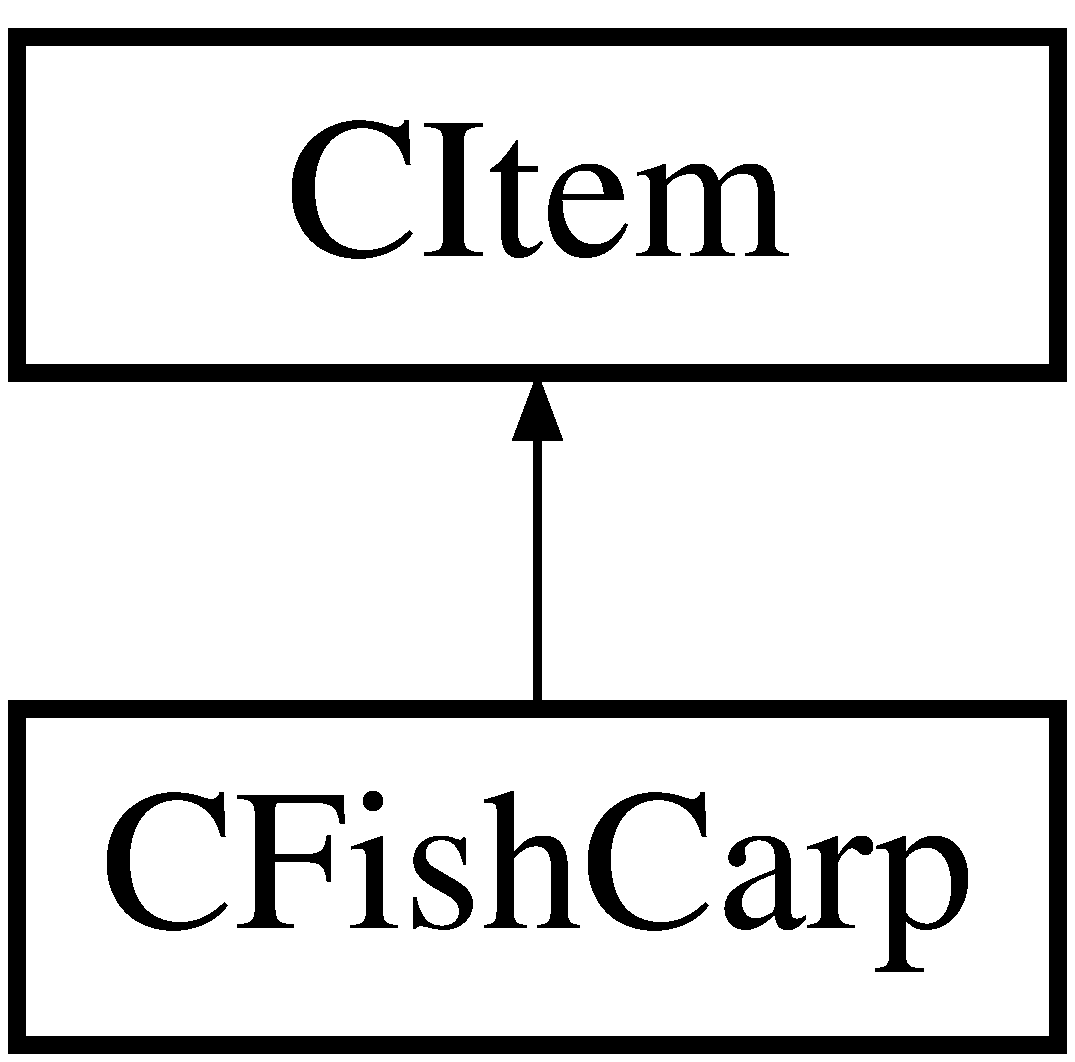
\includegraphics[height=2.000000cm]{class_c_fish_carp}
\end{center}
\end{figure}
\subsection*{Public Member Functions}
\begin{DoxyCompactItemize}
\item 
\hyperlink{class_c_fish_carp_a9bc5ff482658f5b8f09e6d71a143a3e8}{C\+Fish\+Carp} (\hyperlink{class_c_aquarium}{C\+Aquarium} $\ast$aquarium)
\begin{DoxyCompactList}\small\item\em Constructor. \end{DoxyCompactList}\item 
\mbox{\Hypertarget{class_c_fish_carp_a847ccf58041fd6f5aabac7e2ecc9c0d3}\label{class_c_fish_carp_a847ccf58041fd6f5aabac7e2ecc9c0d3}} 
\hyperlink{class_c_fish_carp_a847ccf58041fd6f5aabac7e2ecc9c0d3}{C\+Fish\+Carp} ()=delete
\begin{DoxyCompactList}\small\item\em Default constructor (disabled) \end{DoxyCompactList}\item 
\mbox{\Hypertarget{class_c_fish_carp_a9e7c1ef8083fab86d02544b785431f94}\label{class_c_fish_carp_a9e7c1ef8083fab86d02544b785431f94}} 
\hyperlink{class_c_fish_carp_a9e7c1ef8083fab86d02544b785431f94}{C\+Fish\+Carp} (const \hyperlink{class_c_fish_carp}{C\+Fish\+Carp} \&)=delete
\begin{DoxyCompactList}\small\item\em Copy constructor (disabled) \end{DoxyCompactList}\item 
virtual \hyperlink{class_c_fish_carp_a5f223a99f88b027ac08287ca18f31444}{$\sim$\+C\+Fish\+Carp} ()
\begin{DoxyCompactList}\small\item\em Destructor. \end{DoxyCompactList}\item 
virtual void \hyperlink{class_c_fish_carp_af0c967b07054d90f7b5c2fbfff9e95fb}{Draw} (Gdiplus\+::\+Graphics $\ast$graphics)
\begin{DoxyCompactList}\small\item\em Draws a carp. \end{DoxyCompactList}\item 
bool \hyperlink{class_c_fish_carp_a8e5c6ea5402085533d7535d4524f7fd6}{Hit\+Test} (int x, int y)
\begin{DoxyCompactList}\small\item\em Test to see if we hit this object with a mouse. \end{DoxyCompactList}\item 
virtual bool \hyperlink{class_c_fish_carp_a16a7a5c00b88e1f2ab3fd2db928bd5aa}{Predator} ()
\begin{DoxyCompactList}\small\item\em Tells if this item is a predator. \end{DoxyCompactList}\end{DoxyCompactItemize}
\subsection*{Additional Inherited Members}


\subsection{Detailed Description}
Implements a nemo fish 

\subsection{Constructor \& Destructor Documentation}
\mbox{\Hypertarget{class_c_fish_carp_a9bc5ff482658f5b8f09e6d71a143a3e8}\label{class_c_fish_carp_a9bc5ff482658f5b8f09e6d71a143a3e8}} 
\index{C\+Fish\+Carp@{C\+Fish\+Carp}!C\+Fish\+Carp@{C\+Fish\+Carp}}
\index{C\+Fish\+Carp@{C\+Fish\+Carp}!C\+Fish\+Carp@{C\+Fish\+Carp}}
\subsubsection{\texorpdfstring{C\+Fish\+Carp()}{CFishCarp()}}
{\footnotesize\ttfamily C\+Fish\+Carp\+::\+C\+Fish\+Carp (\begin{DoxyParamCaption}\item[{\hyperlink{class_c_aquarium}{C\+Aquarium} $\ast$}]{aquarium }\end{DoxyParamCaption})}



Constructor. 

Constructor 
\begin{DoxyParams}{Parameters}
{\em aquarium} & The aquarium this is a member of \\
\hline
\end{DoxyParams}
\mbox{\Hypertarget{class_c_fish_carp_a5f223a99f88b027ac08287ca18f31444}\label{class_c_fish_carp_a5f223a99f88b027ac08287ca18f31444}} 
\index{C\+Fish\+Carp@{C\+Fish\+Carp}!````~C\+Fish\+Carp@{$\sim$\+C\+Fish\+Carp}}
\index{````~C\+Fish\+Carp@{$\sim$\+C\+Fish\+Carp}!C\+Fish\+Carp@{C\+Fish\+Carp}}
\subsubsection{\texorpdfstring{$\sim$\+C\+Fish\+Carp()}{~CFishCarp()}}
{\footnotesize\ttfamily C\+Fish\+Carp\+::$\sim$\+C\+Fish\+Carp (\begin{DoxyParamCaption}{ }\end{DoxyParamCaption})\hspace{0.3cm}{\ttfamily [virtual]}}



Destructor. 

Destructor 

\subsection{Member Function Documentation}
\mbox{\Hypertarget{class_c_fish_carp_af0c967b07054d90f7b5c2fbfff9e95fb}\label{class_c_fish_carp_af0c967b07054d90f7b5c2fbfff9e95fb}} 
\index{C\+Fish\+Carp@{C\+Fish\+Carp}!Draw@{Draw}}
\index{Draw@{Draw}!C\+Fish\+Carp@{C\+Fish\+Carp}}
\subsubsection{\texorpdfstring{Draw()}{Draw()}}
{\footnotesize\ttfamily void C\+Fish\+Carp\+::\+Draw (\begin{DoxyParamCaption}\item[{Gdiplus\+::\+Graphics $\ast$}]{graphics }\end{DoxyParamCaption})\hspace{0.3cm}{\ttfamily [virtual]}}



Draws a carp. 

Draw our fish 
\begin{DoxyParams}{Parameters}
{\em graphics} & The graphics context to draw on \\
\hline
\end{DoxyParams}


Implements \hyperlink{class_c_item_a7ef8448d0c4bc53d0f1943a4dc817f6f}{C\+Item}.

\mbox{\Hypertarget{class_c_fish_carp_a8e5c6ea5402085533d7535d4524f7fd6}\label{class_c_fish_carp_a8e5c6ea5402085533d7535d4524f7fd6}} 
\index{C\+Fish\+Carp@{C\+Fish\+Carp}!Hit\+Test@{Hit\+Test}}
\index{Hit\+Test@{Hit\+Test}!C\+Fish\+Carp@{C\+Fish\+Carp}}
\subsubsection{\texorpdfstring{Hit\+Test()}{HitTest()}}
{\footnotesize\ttfamily bool C\+Fish\+Carp\+::\+Hit\+Test (\begin{DoxyParamCaption}\item[{int}]{x,  }\item[{int}]{y }\end{DoxyParamCaption})\hspace{0.3cm}{\ttfamily [virtual]}}



Test to see if we hit this object with a mouse. 

Test to see if we hit this object with a mouse. 
\begin{DoxyParams}{Parameters}
{\em x} & X position to test \\
\hline
{\em y} & Y position to test \\
\hline
\end{DoxyParams}
\begin{DoxyReturn}{Returns}
true if hit. 
\end{DoxyReturn}


Implements \hyperlink{class_c_item_a8bd4f5e3f2eb2487125dd435719484e8}{C\+Item}.

\mbox{\Hypertarget{class_c_fish_carp_a16a7a5c00b88e1f2ab3fd2db928bd5aa}\label{class_c_fish_carp_a16a7a5c00b88e1f2ab3fd2db928bd5aa}} 
\index{C\+Fish\+Carp@{C\+Fish\+Carp}!Predator@{Predator}}
\index{Predator@{Predator}!C\+Fish\+Carp@{C\+Fish\+Carp}}
\subsubsection{\texorpdfstring{Predator()}{Predator()}}
{\footnotesize\ttfamily bool C\+Fish\+Carp\+::\+Predator (\begin{DoxyParamCaption}{ }\end{DoxyParamCaption})\hspace{0.3cm}{\ttfamily [virtual]}}



Tells if this item is a predator. 

Tells if item is a predator \begin{DoxyReturn}{Returns}
true if a predator 
\end{DoxyReturn}


Reimplemented from \hyperlink{class_c_item_af4f25e99aaf4b27ed6bdc5ff70b75c11}{C\+Item}.



The documentation for this class was generated from the following files\+:\begin{DoxyCompactItemize}
\item 
\hyperlink{_fish_carp_8h}{Fish\+Carp.\+h}\item 
\hyperlink{_fish_carp_8cpp}{Fish\+Carp.\+cpp}\end{DoxyCompactItemize}

\hypertarget{class_c_fish_magikarp}{}\section{C\+Fish\+Magikarp Class Reference}
\label{class_c_fish_magikarp}\index{C\+Fish\+Magikarp@{C\+Fish\+Magikarp}}


{\ttfamily \#include $<$Fish\+Magikarp.\+h$>$}

Inheritance diagram for C\+Fish\+Magikarp\+:\begin{figure}[H]
\begin{center}
\leavevmode
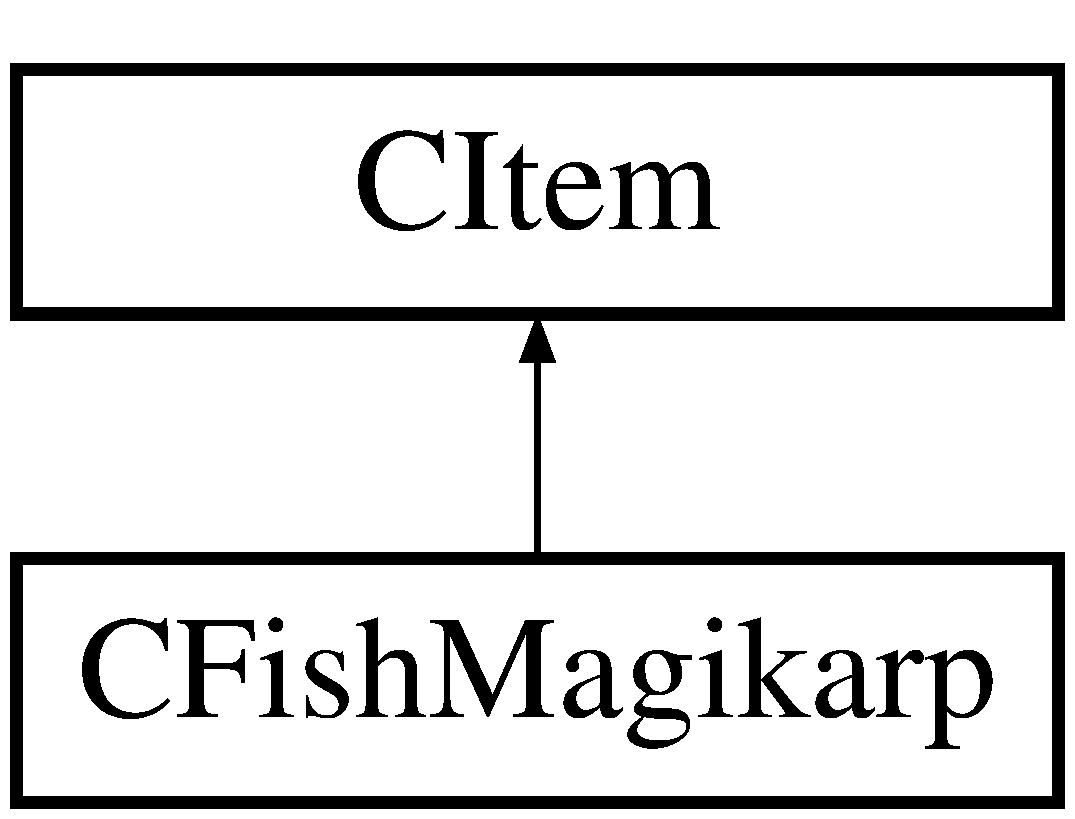
\includegraphics[height=2.000000cm]{class_c_fish_magikarp}
\end{center}
\end{figure}
\subsection*{Public Member Functions}
\begin{DoxyCompactItemize}
\item 
\hyperlink{class_c_fish_magikarp_a364e91206c27040f653fa6c1bc831765}{C\+Fish\+Magikarp} (\hyperlink{class_c_aquarium}{C\+Aquarium} $\ast$aquarium)
\begin{DoxyCompactList}\small\item\em Constructor. \end{DoxyCompactList}\item 
\mbox{\Hypertarget{class_c_fish_magikarp_a16485d202082b7ad5f1f84182f8d0caa}\label{class_c_fish_magikarp_a16485d202082b7ad5f1f84182f8d0caa}} 
\hyperlink{class_c_fish_magikarp_a16485d202082b7ad5f1f84182f8d0caa}{C\+Fish\+Magikarp} ()=delete
\begin{DoxyCompactList}\small\item\em Default constructor (disabled) \end{DoxyCompactList}\item 
\mbox{\Hypertarget{class_c_fish_magikarp_a75df5f848dad873efb158dd3f2bcbb51}\label{class_c_fish_magikarp_a75df5f848dad873efb158dd3f2bcbb51}} 
\hyperlink{class_c_fish_magikarp_a75df5f848dad873efb158dd3f2bcbb51}{C\+Fish\+Magikarp} (const \hyperlink{class_c_fish_magikarp}{C\+Fish\+Magikarp} \&)=delete
\begin{DoxyCompactList}\small\item\em Copy constructor (disabled) \end{DoxyCompactList}\item 
virtual \hyperlink{class_c_fish_magikarp_a6e859fe9c79b553c6b94e110d843e4f9}{$\sim$\+C\+Fish\+Magikarp} ()
\begin{DoxyCompactList}\small\item\em Destructor. \end{DoxyCompactList}\item 
virtual void \hyperlink{class_c_fish_magikarp_acb88cf3659f4cebd4784e7039b541c33}{Draw} (Gdiplus\+::\+Graphics $\ast$graphics)
\begin{DoxyCompactList}\small\item\em Draws a magikarp. \end{DoxyCompactList}\item 
bool \hyperlink{class_c_fish_magikarp_ad23ff73aff08103618b8162dcaaf01b6}{Hit\+Test} (int x, int y)
\begin{DoxyCompactList}\small\item\em Test to see if we hit this object with a mouse. \end{DoxyCompactList}\end{DoxyCompactItemize}
\subsection*{Additional Inherited Members}


\subsection{Detailed Description}
Implements a Magikarp 

\subsection{Constructor \& Destructor Documentation}
\mbox{\Hypertarget{class_c_fish_magikarp_a364e91206c27040f653fa6c1bc831765}\label{class_c_fish_magikarp_a364e91206c27040f653fa6c1bc831765}} 
\index{C\+Fish\+Magikarp@{C\+Fish\+Magikarp}!C\+Fish\+Magikarp@{C\+Fish\+Magikarp}}
\index{C\+Fish\+Magikarp@{C\+Fish\+Magikarp}!C\+Fish\+Magikarp@{C\+Fish\+Magikarp}}
\subsubsection{\texorpdfstring{C\+Fish\+Magikarp()}{CFishMagikarp()}}
{\footnotesize\ttfamily C\+Fish\+Magikarp\+::\+C\+Fish\+Magikarp (\begin{DoxyParamCaption}\item[{\hyperlink{class_c_aquarium}{C\+Aquarium} $\ast$}]{aquarium }\end{DoxyParamCaption})}



Constructor. 

Constructor 
\begin{DoxyParams}{Parameters}
{\em aquarium} & The aquarium this is a member of \\
\hline
\end{DoxyParams}
\mbox{\Hypertarget{class_c_fish_magikarp_a6e859fe9c79b553c6b94e110d843e4f9}\label{class_c_fish_magikarp_a6e859fe9c79b553c6b94e110d843e4f9}} 
\index{C\+Fish\+Magikarp@{C\+Fish\+Magikarp}!````~C\+Fish\+Magikarp@{$\sim$\+C\+Fish\+Magikarp}}
\index{````~C\+Fish\+Magikarp@{$\sim$\+C\+Fish\+Magikarp}!C\+Fish\+Magikarp@{C\+Fish\+Magikarp}}
\subsubsection{\texorpdfstring{$\sim$\+C\+Fish\+Magikarp()}{~CFishMagikarp()}}
{\footnotesize\ttfamily C\+Fish\+Magikarp\+::$\sim$\+C\+Fish\+Magikarp (\begin{DoxyParamCaption}{ }\end{DoxyParamCaption})\hspace{0.3cm}{\ttfamily [virtual]}}



Destructor. 

Destructor 

\subsection{Member Function Documentation}
\mbox{\Hypertarget{class_c_fish_magikarp_acb88cf3659f4cebd4784e7039b541c33}\label{class_c_fish_magikarp_acb88cf3659f4cebd4784e7039b541c33}} 
\index{C\+Fish\+Magikarp@{C\+Fish\+Magikarp}!Draw@{Draw}}
\index{Draw@{Draw}!C\+Fish\+Magikarp@{C\+Fish\+Magikarp}}
\subsubsection{\texorpdfstring{Draw()}{Draw()}}
{\footnotesize\ttfamily void C\+Fish\+Magikarp\+::\+Draw (\begin{DoxyParamCaption}\item[{Gdiplus\+::\+Graphics $\ast$}]{graphics }\end{DoxyParamCaption})\hspace{0.3cm}{\ttfamily [virtual]}}



Draws a magikarp. 

Draw our fish 
\begin{DoxyParams}{Parameters}
{\em graphics} & The graphics context to draw on \\
\hline
\end{DoxyParams}


Implements \hyperlink{class_c_item_a7ef8448d0c4bc53d0f1943a4dc817f6f}{C\+Item}.

\mbox{\Hypertarget{class_c_fish_magikarp_ad23ff73aff08103618b8162dcaaf01b6}\label{class_c_fish_magikarp_ad23ff73aff08103618b8162dcaaf01b6}} 
\index{C\+Fish\+Magikarp@{C\+Fish\+Magikarp}!Hit\+Test@{Hit\+Test}}
\index{Hit\+Test@{Hit\+Test}!C\+Fish\+Magikarp@{C\+Fish\+Magikarp}}
\subsubsection{\texorpdfstring{Hit\+Test()}{HitTest()}}
{\footnotesize\ttfamily bool C\+Fish\+Magikarp\+::\+Hit\+Test (\begin{DoxyParamCaption}\item[{int}]{x,  }\item[{int}]{y }\end{DoxyParamCaption})\hspace{0.3cm}{\ttfamily [virtual]}}



Test to see if we hit this object with a mouse. 

Test to see if we hit this object with a mouse. 
\begin{DoxyParams}{Parameters}
{\em x} & X position to test \\
\hline
{\em y} & Y position to test \\
\hline
\end{DoxyParams}
\begin{DoxyReturn}{Returns}
true if hit. 
\end{DoxyReturn}


Implements \hyperlink{class_c_item_a8bd4f5e3f2eb2487125dd435719484e8}{C\+Item}.



The documentation for this class was generated from the following files\+:\begin{DoxyCompactItemize}
\item 
\hyperlink{_fish_magikarp_8h}{Fish\+Magikarp.\+h}\item 
\hyperlink{_fish_magikarp_8cpp}{Fish\+Magikarp.\+cpp}\end{DoxyCompactItemize}

\hypertarget{class_c_fish_nemo}{}\section{C\+Fish\+Nemo Class Reference}
\label{class_c_fish_nemo}\index{C\+Fish\+Nemo@{C\+Fish\+Nemo}}


{\ttfamily \#include $<$Fish\+Nemo.\+h$>$}

Inheritance diagram for C\+Fish\+Nemo\+:\begin{figure}[H]
\begin{center}
\leavevmode
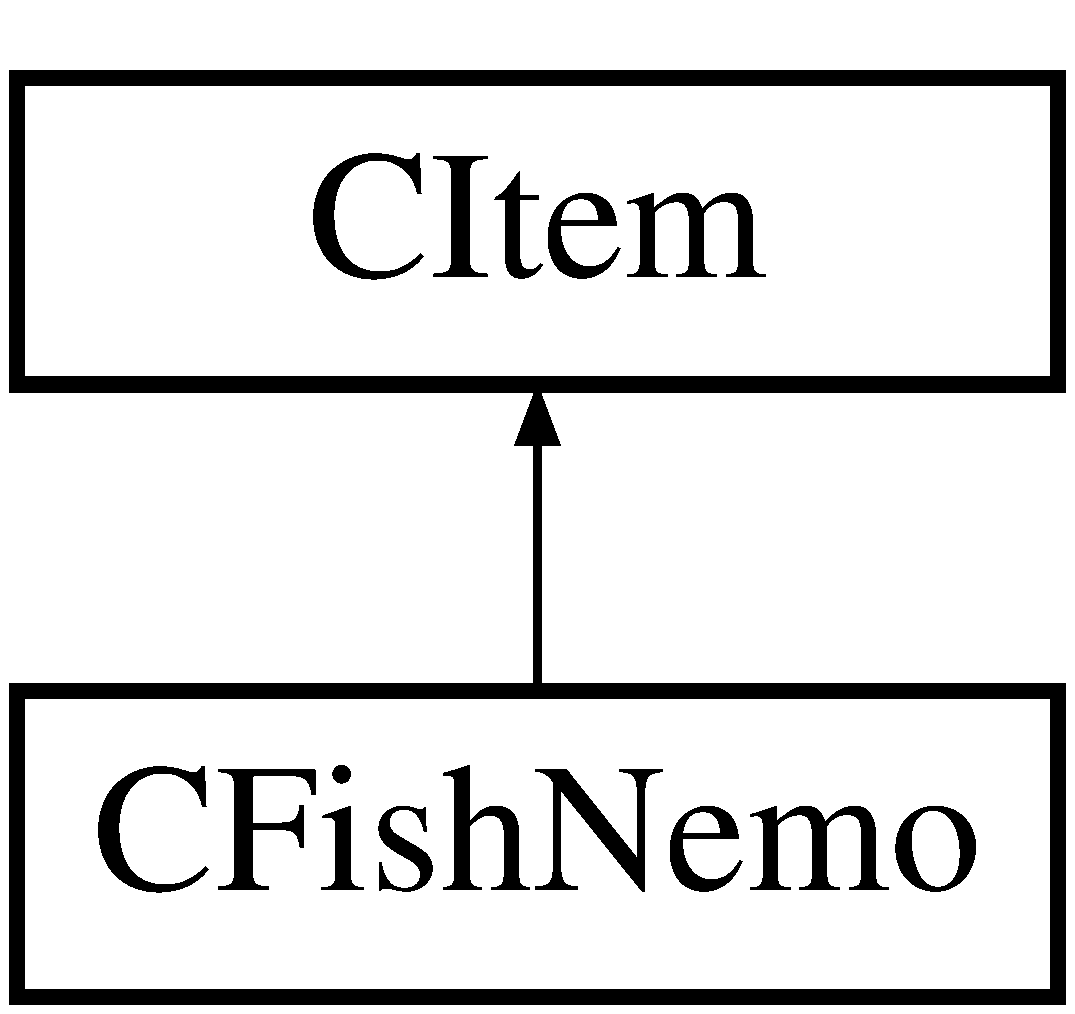
\includegraphics[height=2.000000cm]{class_c_fish_nemo}
\end{center}
\end{figure}
\subsection*{Public Member Functions}
\begin{DoxyCompactItemize}
\item 
\hyperlink{class_c_fish_nemo_ab5cc8d119b0c9d8dc62a0e2b6f6e731d}{C\+Fish\+Nemo} (\hyperlink{class_c_aquarium}{C\+Aquarium} $\ast$aquarium)
\begin{DoxyCompactList}\small\item\em Constructor. \end{DoxyCompactList}\item 
\mbox{\Hypertarget{class_c_fish_nemo_abb741271acb8aeb31fea93f5048d171e}\label{class_c_fish_nemo_abb741271acb8aeb31fea93f5048d171e}} 
\hyperlink{class_c_fish_nemo_abb741271acb8aeb31fea93f5048d171e}{C\+Fish\+Nemo} ()=delete
\begin{DoxyCompactList}\small\item\em Default constructor (disabled) \end{DoxyCompactList}\item 
\mbox{\Hypertarget{class_c_fish_nemo_a354e7fcb47bbf51c30c148c77dfbb59b}\label{class_c_fish_nemo_a354e7fcb47bbf51c30c148c77dfbb59b}} 
\hyperlink{class_c_fish_nemo_a354e7fcb47bbf51c30c148c77dfbb59b}{C\+Fish\+Nemo} (const \hyperlink{class_c_fish_nemo}{C\+Fish\+Nemo} \&)=delete
\begin{DoxyCompactList}\small\item\em Copy constructor (disabled) \end{DoxyCompactList}\item 
virtual \hyperlink{class_c_fish_nemo_ac37da91b4738144d3b47674450861b26}{$\sim$\+C\+Fish\+Nemo} ()
\begin{DoxyCompactList}\small\item\em Destructor. \end{DoxyCompactList}\item 
virtual void \hyperlink{class_c_fish_nemo_a56389067cff39be91a796f42529458d3}{Draw} (Gdiplus\+::\+Graphics $\ast$graphics)
\begin{DoxyCompactList}\small\item\em Draws nemo. \end{DoxyCompactList}\item 
bool \hyperlink{class_c_fish_nemo_a7ab85960d0a36a80cd6bf7fb78afe0ee}{Hit\+Test} (int x, int y)
\begin{DoxyCompactList}\small\item\em Test to see if we hit this object with a mouse. \end{DoxyCompactList}\end{DoxyCompactItemize}
\subsection*{Additional Inherited Members}


\subsection{Detailed Description}
Implements a nemo fish 

\subsection{Constructor \& Destructor Documentation}
\mbox{\Hypertarget{class_c_fish_nemo_ab5cc8d119b0c9d8dc62a0e2b6f6e731d}\label{class_c_fish_nemo_ab5cc8d119b0c9d8dc62a0e2b6f6e731d}} 
\index{C\+Fish\+Nemo@{C\+Fish\+Nemo}!C\+Fish\+Nemo@{C\+Fish\+Nemo}}
\index{C\+Fish\+Nemo@{C\+Fish\+Nemo}!C\+Fish\+Nemo@{C\+Fish\+Nemo}}
\subsubsection{\texorpdfstring{C\+Fish\+Nemo()}{CFishNemo()}}
{\footnotesize\ttfamily C\+Fish\+Nemo\+::\+C\+Fish\+Nemo (\begin{DoxyParamCaption}\item[{\hyperlink{class_c_aquarium}{C\+Aquarium} $\ast$}]{aquarium }\end{DoxyParamCaption})}



Constructor. 

Constructor 
\begin{DoxyParams}{Parameters}
{\em aquarium} & The aquarium this is a member of \\
\hline
\end{DoxyParams}
\mbox{\Hypertarget{class_c_fish_nemo_ac37da91b4738144d3b47674450861b26}\label{class_c_fish_nemo_ac37da91b4738144d3b47674450861b26}} 
\index{C\+Fish\+Nemo@{C\+Fish\+Nemo}!````~C\+Fish\+Nemo@{$\sim$\+C\+Fish\+Nemo}}
\index{````~C\+Fish\+Nemo@{$\sim$\+C\+Fish\+Nemo}!C\+Fish\+Nemo@{C\+Fish\+Nemo}}
\subsubsection{\texorpdfstring{$\sim$\+C\+Fish\+Nemo()}{~CFishNemo()}}
{\footnotesize\ttfamily C\+Fish\+Nemo\+::$\sim$\+C\+Fish\+Nemo (\begin{DoxyParamCaption}{ }\end{DoxyParamCaption})\hspace{0.3cm}{\ttfamily [virtual]}}



Destructor. 

Destructor 

\subsection{Member Function Documentation}
\mbox{\Hypertarget{class_c_fish_nemo_a56389067cff39be91a796f42529458d3}\label{class_c_fish_nemo_a56389067cff39be91a796f42529458d3}} 
\index{C\+Fish\+Nemo@{C\+Fish\+Nemo}!Draw@{Draw}}
\index{Draw@{Draw}!C\+Fish\+Nemo@{C\+Fish\+Nemo}}
\subsubsection{\texorpdfstring{Draw()}{Draw()}}
{\footnotesize\ttfamily void C\+Fish\+Nemo\+::\+Draw (\begin{DoxyParamCaption}\item[{Gdiplus\+::\+Graphics $\ast$}]{graphics }\end{DoxyParamCaption})\hspace{0.3cm}{\ttfamily [virtual]}}



Draws nemo. 

Draw our fish 
\begin{DoxyParams}{Parameters}
{\em graphics} & The graphics context to draw on \\
\hline
\end{DoxyParams}


Implements \hyperlink{class_c_item_a7ef8448d0c4bc53d0f1943a4dc817f6f}{C\+Item}.

\mbox{\Hypertarget{class_c_fish_nemo_a7ab85960d0a36a80cd6bf7fb78afe0ee}\label{class_c_fish_nemo_a7ab85960d0a36a80cd6bf7fb78afe0ee}} 
\index{C\+Fish\+Nemo@{C\+Fish\+Nemo}!Hit\+Test@{Hit\+Test}}
\index{Hit\+Test@{Hit\+Test}!C\+Fish\+Nemo@{C\+Fish\+Nemo}}
\subsubsection{\texorpdfstring{Hit\+Test()}{HitTest()}}
{\footnotesize\ttfamily bool C\+Fish\+Nemo\+::\+Hit\+Test (\begin{DoxyParamCaption}\item[{int}]{x,  }\item[{int}]{y }\end{DoxyParamCaption})\hspace{0.3cm}{\ttfamily [virtual]}}



Test to see if we hit this object with a mouse. 

Test to see if we hit this object with a mouse. 
\begin{DoxyParams}{Parameters}
{\em x} & X position to test \\
\hline
{\em y} & Y position to test \\
\hline
\end{DoxyParams}
\begin{DoxyReturn}{Returns}
true if hit. 
\end{DoxyReturn}


Implements \hyperlink{class_c_item_a8bd4f5e3f2eb2487125dd435719484e8}{C\+Item}.



The documentation for this class was generated from the following files\+:\begin{DoxyCompactItemize}
\item 
\hyperlink{_fish_nemo_8h}{Fish\+Nemo.\+h}\item 
\hyperlink{_fish_nemo_8cpp}{Fish\+Nemo.\+cpp}\end{DoxyCompactItemize}

\hypertarget{class_c_item}{}\section{C\+Item Class Reference}
\label{class_c_item}\index{C\+Item@{C\+Item}}


{\ttfamily \#include $<$Item.\+h$>$}

Inheritance diagram for C\+Item\+:\begin{figure}[H]
\begin{center}
\leavevmode
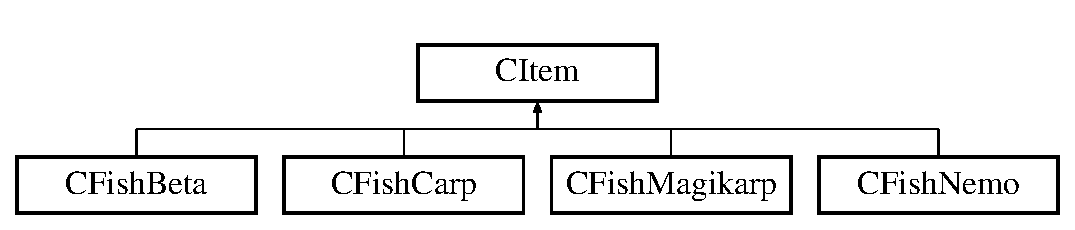
\includegraphics[height=2.000000cm]{class_c_item}
\end{center}
\end{figure}
\subsection*{Public Member Functions}
\begin{DoxyCompactItemize}
\item 
\mbox{\Hypertarget{class_c_item_ac2ea847c008cf8d1de92c870c8f8262f}\label{class_c_item_ac2ea847c008cf8d1de92c870c8f8262f}} 
\hyperlink{class_c_item_ac2ea847c008cf8d1de92c870c8f8262f}{C\+Item} ()=delete
\begin{DoxyCompactList}\small\item\em Default constructor (disabled) \end{DoxyCompactList}\item 
\mbox{\Hypertarget{class_c_item_a7d6042bbb9a571d2dc1d1f89016a97c8}\label{class_c_item_a7d6042bbb9a571d2dc1d1f89016a97c8}} 
\hyperlink{class_c_item_a7d6042bbb9a571d2dc1d1f89016a97c8}{C\+Item} (const \hyperlink{class_c_item}{C\+Item} \&)=delete
\begin{DoxyCompactList}\small\item\em Copy constructor (disabled) \end{DoxyCompactList}\item 
virtual \hyperlink{class_c_item_a2487c6e822ed0e850544f1745b43f584}{$\sim$\+C\+Item} ()
\begin{DoxyCompactList}\small\item\em Destructor. \end{DoxyCompactList}\item 
double \hyperlink{class_c_item_a394d38a058fc53f0e958ca52248560c8}{GetX} () const
\item 
double \hyperlink{class_c_item_ac0fe6be80f8ef19854d7f41b4803f658}{GetY} () const
\item 
void \hyperlink{class_c_item_a9c194f3f08e515853600cecca3e6d319}{Set\+Location} (double x, double y)
\item 
virtual void \hyperlink{class_c_item_a7ef8448d0c4bc53d0f1943a4dc817f6f}{Draw} (Gdiplus\+::\+Graphics $\ast$graphics)=0
\item 
virtual bool \hyperlink{class_c_item_a8bd4f5e3f2eb2487125dd435719484e8}{Hit\+Test} (int x, int y)=0
\item 
virtual bool \hyperlink{class_c_item_af4f25e99aaf4b27ed6bdc5ff70b75c11}{Predator} ()
\begin{DoxyCompactList}\small\item\em Tells whether or not an item is a predator. \end{DoxyCompactList}\end{DoxyCompactItemize}
\subsection*{Protected Member Functions}
\begin{DoxyCompactItemize}
\item 
\hyperlink{class_c_item_a665b3fa4628b43e69b1d7f2b9529882b}{C\+Item} (\hyperlink{class_c_aquarium}{C\+Aquarium} $\ast$aquarium)
\begin{DoxyCompactList}\small\item\em Constructor. \end{DoxyCompactList}\end{DoxyCompactItemize}


\subsection{Detailed Description}
Base class for any item in our aquarium. 

\subsection{Constructor \& Destructor Documentation}
\mbox{\Hypertarget{class_c_item_a2487c6e822ed0e850544f1745b43f584}\label{class_c_item_a2487c6e822ed0e850544f1745b43f584}} 
\index{C\+Item@{C\+Item}!````~C\+Item@{$\sim$\+C\+Item}}
\index{````~C\+Item@{$\sim$\+C\+Item}!C\+Item@{C\+Item}}
\subsubsection{\texorpdfstring{$\sim$\+C\+Item()}{~CItem()}}
{\footnotesize\ttfamily C\+Item\+::$\sim$\+C\+Item (\begin{DoxyParamCaption}{ }\end{DoxyParamCaption})\hspace{0.3cm}{\ttfamily [virtual]}}



Destructor. 

Destructor \mbox{\Hypertarget{class_c_item_a665b3fa4628b43e69b1d7f2b9529882b}\label{class_c_item_a665b3fa4628b43e69b1d7f2b9529882b}} 
\index{C\+Item@{C\+Item}!C\+Item@{C\+Item}}
\index{C\+Item@{C\+Item}!C\+Item@{C\+Item}}
\subsubsection{\texorpdfstring{C\+Item()}{CItem()}}
{\footnotesize\ttfamily C\+Item\+::\+C\+Item (\begin{DoxyParamCaption}\item[{\hyperlink{class_c_aquarium}{C\+Aquarium} $\ast$}]{aquarium }\end{DoxyParamCaption})\hspace{0.3cm}{\ttfamily [protected]}}



Constructor. 

Constructor 
\begin{DoxyParams}{Parameters}
{\em aquarium} & The aquarium this item is a member of \\
\hline
\end{DoxyParams}


\subsection{Member Function Documentation}
\mbox{\Hypertarget{class_c_item_a7ef8448d0c4bc53d0f1943a4dc817f6f}\label{class_c_item_a7ef8448d0c4bc53d0f1943a4dc817f6f}} 
\index{C\+Item@{C\+Item}!Draw@{Draw}}
\index{Draw@{Draw}!C\+Item@{C\+Item}}
\subsubsection{\texorpdfstring{Draw()}{Draw()}}
{\footnotesize\ttfamily virtual void C\+Item\+::\+Draw (\begin{DoxyParamCaption}\item[{Gdiplus\+::\+Graphics $\ast$}]{graphics }\end{DoxyParamCaption})\hspace{0.3cm}{\ttfamily [pure virtual]}}

Draw this item 
\begin{DoxyParams}{Parameters}
{\em graphics} & Graphics device to draw on \\
\hline
\end{DoxyParams}


Implemented in \hyperlink{class_c_fish_beta_ae2effbff7b98bb3cd6e1070d61d5366e}{C\+Fish\+Beta}, \hyperlink{class_c_fish_carp_af0c967b07054d90f7b5c2fbfff9e95fb}{C\+Fish\+Carp}, \hyperlink{class_c_fish_magikarp_acb88cf3659f4cebd4784e7039b541c33}{C\+Fish\+Magikarp}, and \hyperlink{class_c_fish_nemo_a56389067cff39be91a796f42529458d3}{C\+Fish\+Nemo}.

\mbox{\Hypertarget{class_c_item_a394d38a058fc53f0e958ca52248560c8}\label{class_c_item_a394d38a058fc53f0e958ca52248560c8}} 
\index{C\+Item@{C\+Item}!GetX@{GetX}}
\index{GetX@{GetX}!C\+Item@{C\+Item}}
\subsubsection{\texorpdfstring{Get\+X()}{GetX()}}
{\footnotesize\ttfamily double C\+Item\+::\+GetX (\begin{DoxyParamCaption}{ }\end{DoxyParamCaption}) const\hspace{0.3cm}{\ttfamily [inline]}}

The X location of the item \begin{DoxyReturn}{Returns}
X location in pixels 
\end{DoxyReturn}
\mbox{\Hypertarget{class_c_item_ac0fe6be80f8ef19854d7f41b4803f658}\label{class_c_item_ac0fe6be80f8ef19854d7f41b4803f658}} 
\index{C\+Item@{C\+Item}!GetY@{GetY}}
\index{GetY@{GetY}!C\+Item@{C\+Item}}
\subsubsection{\texorpdfstring{Get\+Y()}{GetY()}}
{\footnotesize\ttfamily double C\+Item\+::\+GetY (\begin{DoxyParamCaption}{ }\end{DoxyParamCaption}) const\hspace{0.3cm}{\ttfamily [inline]}}

The Y location of the item \begin{DoxyReturn}{Returns}
Y location in pixels 
\end{DoxyReturn}
\mbox{\Hypertarget{class_c_item_a8bd4f5e3f2eb2487125dd435719484e8}\label{class_c_item_a8bd4f5e3f2eb2487125dd435719484e8}} 
\index{C\+Item@{C\+Item}!Hit\+Test@{Hit\+Test}}
\index{Hit\+Test@{Hit\+Test}!C\+Item@{C\+Item}}
\subsubsection{\texorpdfstring{Hit\+Test()}{HitTest()}}
{\footnotesize\ttfamily virtual bool C\+Item\+::\+Hit\+Test (\begin{DoxyParamCaption}\item[{int}]{x,  }\item[{int}]{y }\end{DoxyParamCaption})\hspace{0.3cm}{\ttfamily [pure virtual]}}

Test this item to see if it has been clicked on 
\begin{DoxyParams}{Parameters}
{\em x} & X location on the aquarium to test \\
\hline
{\em y} & Y location on the aquarium to test \\
\hline
\end{DoxyParams}
\begin{DoxyReturn}{Returns}
true if clicked on 
\end{DoxyReturn}


Implemented in \hyperlink{class_c_fish_beta_a5bdd3d07a57ca1f01a7f2c5c00e0a662}{C\+Fish\+Beta}, \hyperlink{class_c_fish_carp_a8e5c6ea5402085533d7535d4524f7fd6}{C\+Fish\+Carp}, \hyperlink{class_c_fish_magikarp_ad23ff73aff08103618b8162dcaaf01b6}{C\+Fish\+Magikarp}, and \hyperlink{class_c_fish_nemo_a7ab85960d0a36a80cd6bf7fb78afe0ee}{C\+Fish\+Nemo}.

\mbox{\Hypertarget{class_c_item_af4f25e99aaf4b27ed6bdc5ff70b75c11}\label{class_c_item_af4f25e99aaf4b27ed6bdc5ff70b75c11}} 
\index{C\+Item@{C\+Item}!Predator@{Predator}}
\index{Predator@{Predator}!C\+Item@{C\+Item}}
\subsubsection{\texorpdfstring{Predator()}{Predator()}}
{\footnotesize\ttfamily bool C\+Item\+::\+Predator (\begin{DoxyParamCaption}{ }\end{DoxyParamCaption})\hspace{0.3cm}{\ttfamily [virtual]}}



Tells whether or not an item is a predator. 

Tells if the item (fish) is a predator \begin{DoxyReturn}{Returns}
false if function not overwritten/predator 
\end{DoxyReturn}


Reimplemented in \hyperlink{class_c_fish_carp_a16a7a5c00b88e1f2ab3fd2db928bd5aa}{C\+Fish\+Carp}.

\mbox{\Hypertarget{class_c_item_a9c194f3f08e515853600cecca3e6d319}\label{class_c_item_a9c194f3f08e515853600cecca3e6d319}} 
\index{C\+Item@{C\+Item}!Set\+Location@{Set\+Location}}
\index{Set\+Location@{Set\+Location}!C\+Item@{C\+Item}}
\subsubsection{\texorpdfstring{Set\+Location()}{SetLocation()}}
{\footnotesize\ttfamily void C\+Item\+::\+Set\+Location (\begin{DoxyParamCaption}\item[{double}]{x,  }\item[{double}]{y }\end{DoxyParamCaption})\hspace{0.3cm}{\ttfamily [inline]}}

Set the item location 
\begin{DoxyParams}{Parameters}
{\em x} & X location \\
\hline
{\em y} & Y location \\
\hline
\end{DoxyParams}


The documentation for this class was generated from the following files\+:\begin{DoxyCompactItemize}
\item 
\hyperlink{_item_8h}{Item.\+h}\item 
\hyperlink{_item_8cpp}{Item.\+cpp}\end{DoxyCompactItemize}

\hypertarget{class_c_main_frame}{}\section{C\+Main\+Frame Class Reference}
\label{class_c_main_frame}\index{C\+Main\+Frame@{C\+Main\+Frame}}
Inheritance diagram for C\+Main\+Frame\+:\begin{figure}[H]
\begin{center}
\leavevmode
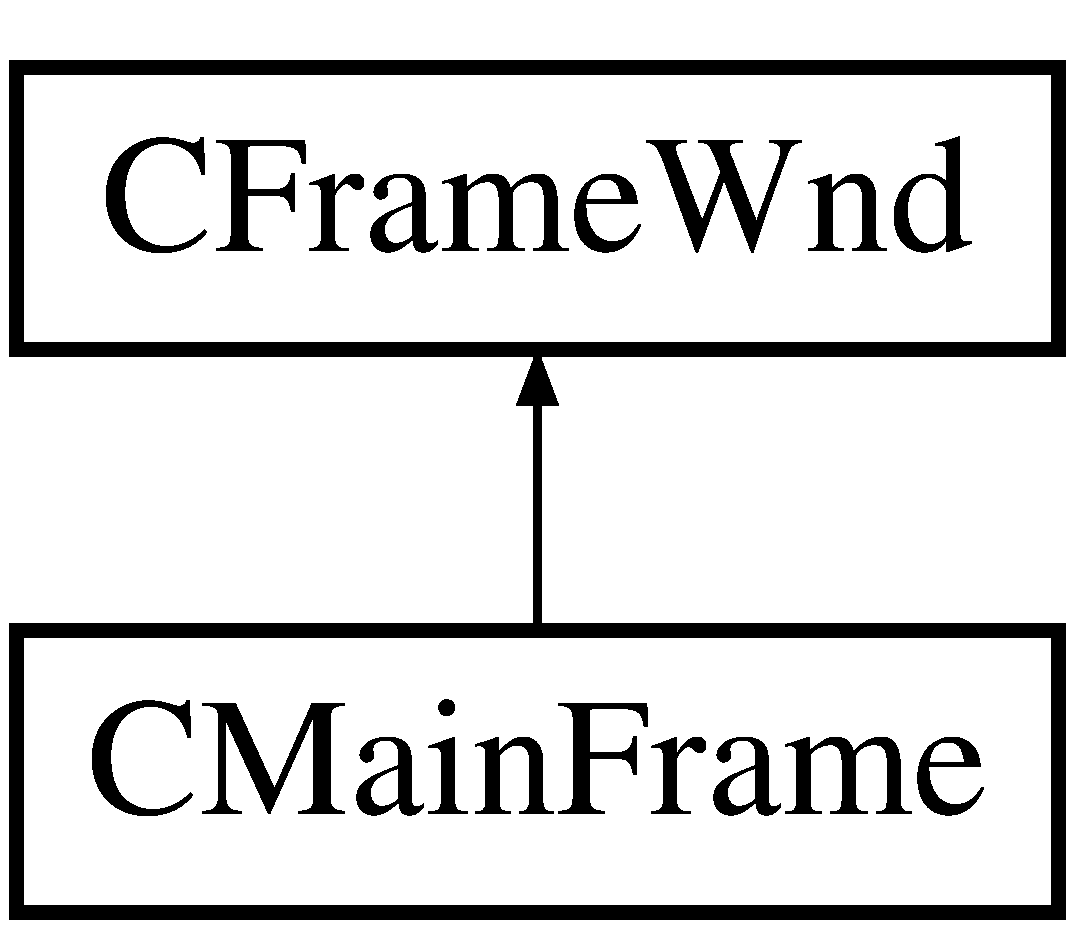
\includegraphics[height=2.000000cm]{class_c_main_frame}
\end{center}
\end{figure}
\subsection*{Public Member Functions}
\begin{DoxyCompactItemize}
\item 
\mbox{\Hypertarget{class_c_main_frame_a549bf677c955c2898c3c683321633c16}\label{class_c_main_frame_a549bf677c955c2898c3c683321633c16}} 
virtual B\+O\+OL {\bfseries Pre\+Create\+Window} (C\+R\+E\+A\+T\+E\+S\+T\+R\+U\+CT \&cs)
\item 
\mbox{\Hypertarget{class_c_main_frame_ade959eb0bab719bf06bb9b18ee407101}\label{class_c_main_frame_ade959eb0bab719bf06bb9b18ee407101}} 
virtual B\+O\+OL {\bfseries On\+Cmd\+Msg} (U\+I\+NT n\+ID, int n\+Code, void $\ast$p\+Extra, A\+F\+X\+\_\+\+C\+M\+D\+H\+A\+N\+D\+L\+E\+R\+I\+N\+FO $\ast$p\+Handler\+Info)
\end{DoxyCompactItemize}
\subsection*{Protected Member Functions}
\begin{DoxyCompactItemize}
\item 
\mbox{\Hypertarget{class_c_main_frame_a48666466fd37412fcaeff75c3b12e0ed}\label{class_c_main_frame_a48666466fd37412fcaeff75c3b12e0ed}} 
afx\+\_\+msg int {\bfseries On\+Create} (L\+P\+C\+R\+E\+A\+T\+E\+S\+T\+R\+U\+CT lp\+Create\+Struct)
\item 
\mbox{\Hypertarget{class_c_main_frame_adc353a3d1fc497fbc009b6d9e6914a82}\label{class_c_main_frame_adc353a3d1fc497fbc009b6d9e6914a82}} 
afx\+\_\+msg void {\bfseries On\+Set\+Focus} (C\+Wnd $\ast$p\+Old\+Wnd)
\end{DoxyCompactItemize}
\subsection*{Protected Attributes}
\begin{DoxyCompactItemize}
\item 
\mbox{\Hypertarget{class_c_main_frame_a73024d794dce2fe918f6b117371c25fc}\label{class_c_main_frame_a73024d794dce2fe918f6b117371c25fc}} 
C\+Tool\+Bar {\bfseries m\+\_\+wnd\+Tool\+Bar}
\item 
\mbox{\Hypertarget{class_c_main_frame_ac01bafc03aee69cf982e6f029b4db6b0}\label{class_c_main_frame_ac01bafc03aee69cf982e6f029b4db6b0}} 
C\+Status\+Bar {\bfseries m\+\_\+wnd\+Status\+Bar}
\item 
\mbox{\Hypertarget{class_c_main_frame_a7c3af9327c496f8c807d578f7a4ef4c5}\label{class_c_main_frame_a7c3af9327c496f8c807d578f7a4ef4c5}} 
\hyperlink{class_c_child_view}{C\+Child\+View} {\bfseries m\+\_\+wnd\+View}
\end{DoxyCompactItemize}


The documentation for this class was generated from the following files\+:\begin{DoxyCompactItemize}
\item 
Main\+Frm.\+h\item 
Main\+Frm.\+cpp\end{DoxyCompactItemize}

\hypertarget{class_c_step2_app}{}\section{C\+Step2\+App Class Reference}
\label{class_c_step2_app}\index{C\+Step2\+App@{C\+Step2\+App}}
Inheritance diagram for C\+Step2\+App\+:\begin{figure}[H]
\begin{center}
\leavevmode
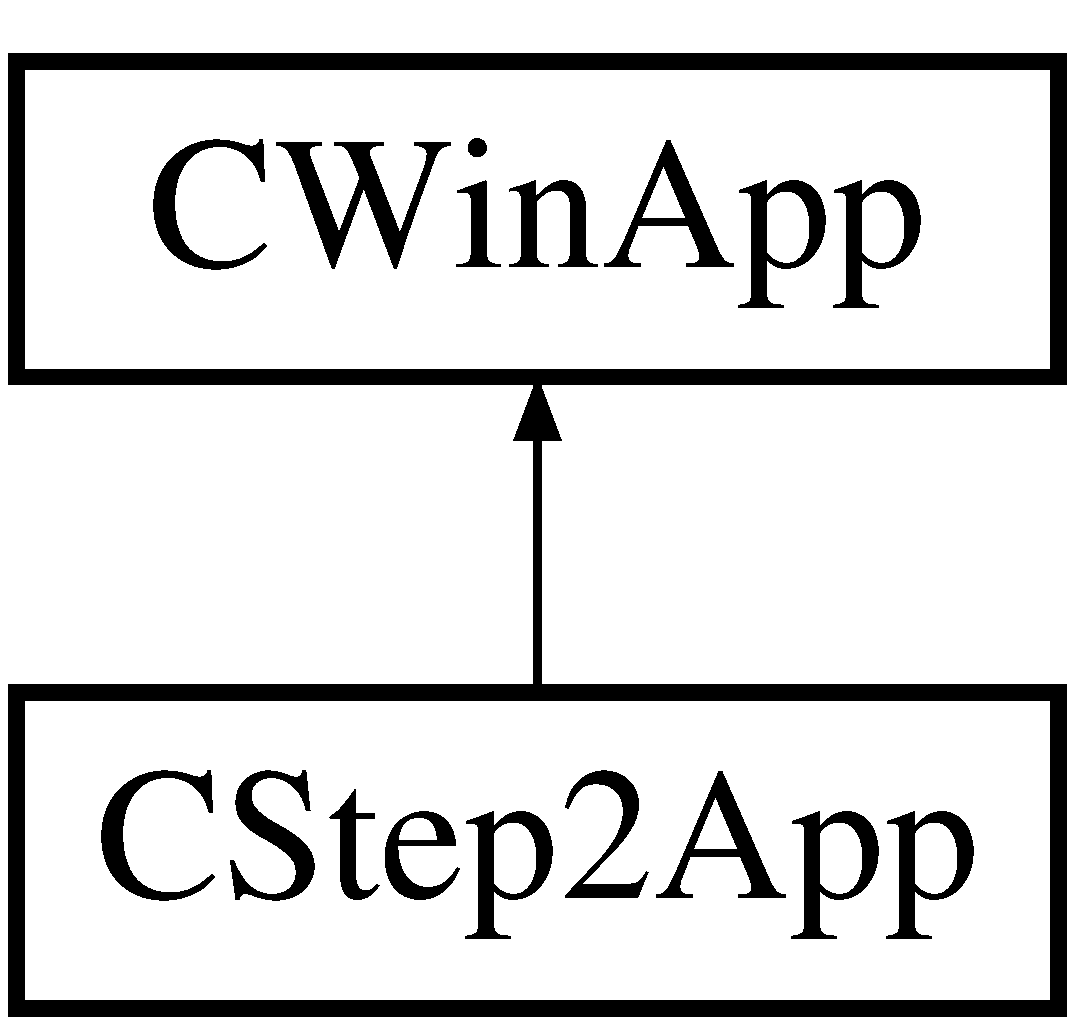
\includegraphics[height=2.000000cm]{class_c_step2_app}
\end{center}
\end{figure}
\subsection*{Public Member Functions}
\begin{DoxyCompactItemize}
\item 
\mbox{\Hypertarget{class_c_step2_app_a4152bf861e6e520eaa173c41a3d9f73d}\label{class_c_step2_app_a4152bf861e6e520eaa173c41a3d9f73d}} 
virtual B\+O\+OL {\bfseries Init\+Instance} ()
\item 
\mbox{\Hypertarget{class_c_step2_app_aad455705e63bb9ae0642be6ca2d2b684}\label{class_c_step2_app_aad455705e63bb9ae0642be6ca2d2b684}} 
virtual int {\bfseries Exit\+Instance} ()
\item 
\mbox{\Hypertarget{class_c_step2_app_a7407f02b1d0628458512c9f35ab2bb50}\label{class_c_step2_app_a7407f02b1d0628458512c9f35ab2bb50}} 
afx\+\_\+msg void {\bfseries On\+App\+About} ()
\end{DoxyCompactItemize}


The documentation for this class was generated from the following files\+:\begin{DoxyCompactItemize}
\item 
Step2.\+h\item 
Step2.\+cpp\end{DoxyCompactItemize}

\chapter{File Documentation}
\hypertarget{_aquarium_8cpp}{}\section{Aquarium.\+cpp File Reference}
\label{_aquarium_8cpp}\index{Aquarium.\+cpp@{Aquarium.\+cpp}}
{\ttfamily \#include \char`\"{}stdafx.\+h\char`\"{}}\newline
{\ttfamily \#include \char`\"{}Aquarium.\+h\char`\"{}}\newline
{\ttfamily \#include \char`\"{}Fish\+Beta.\+h\char`\"{}}\newline
{\ttfamily \#include $<$algorithm$>$}\newline


\subsection{Detailed Description}
\begin{DoxyAuthor}{Author}
Romi Yun 
\end{DoxyAuthor}

\hypertarget{_aquarium_8h}{}\section{Aquarium.\+h File Reference}
\label{_aquarium_8h}\index{Aquarium.\+h@{Aquarium.\+h}}
{\ttfamily \#include $<$memory$>$}\newline
{\ttfamily \#include $<$vector$>$}\newline
\subsection*{Classes}
\begin{DoxyCompactItemize}
\item 
class \hyperlink{class_c_aquarium}{C\+Aquarium}
\end{DoxyCompactItemize}


\subsection{Detailed Description}
\begin{DoxyAuthor}{Author}
Romi Yun
\end{DoxyAuthor}
Class that represents an aquarium. 
\hypertarget{_child_view_8cpp}{}\section{Child\+View.\+cpp File Reference}
\label{_child_view_8cpp}\index{Child\+View.\+cpp@{Child\+View.\+cpp}}
{\ttfamily \#include \char`\"{}stdafx.\+h\char`\"{}}\newline
{\ttfamily \#include \char`\"{}Step2.\+h\char`\"{}}\newline
{\ttfamily \#include \char`\"{}Child\+View.\+h\char`\"{}}\newline
{\ttfamily \#include \char`\"{}Fish\+Beta.\+h\char`\"{}}\newline
{\ttfamily \#include \char`\"{}Fish\+Magikarp.\+h\char`\"{}}\newline
{\ttfamily \#include \char`\"{}Fish\+Nemo.\+h\char`\"{}}\newline
{\ttfamily \#include \char`\"{}Fish\+Carp.\+h\char`\"{}}\newline
{\ttfamily \#include \char`\"{}Double\+Buffer\+D\+C.\+h\char`\"{}}\newline
\subsection*{Functions}
\begin{DoxyCompactItemize}
\item 
\mbox{\Hypertarget{_child_view_8cpp_a559230bd2db2a07315c7be9eb50ad948}\label{_child_view_8cpp_a559230bd2db2a07315c7be9eb50ad948}} 
{\bfseries B\+E\+G\+I\+N\+\_\+\+M\+E\+S\+S\+A\+G\+E\+\_\+\+M\+AP} (\hyperlink{class_c_child_view}{C\+Child\+View}, C\+Wnd) O\+N\+\_\+\+W\+M\+\_\+\+P\+A\+I\+NT() O\+N\+\_\+\+C\+O\+M\+M\+A\+ND(I\+D\+\_\+\+A\+D\+D\+F\+I\+S\+H\+\_\+\+B\+E\+T\+A\+F\+I\+SH
\item 
\mbox{\Hypertarget{_child_view_8cpp_a81af5327ded229a60affa1b48191b4cc}\label{_child_view_8cpp_a81af5327ded229a60affa1b48191b4cc}} 
\&\hyperlink{class_c_child_view_a3d54ea142fb2facf2f19fa6772346667}{C\+Child\+View\+::\+On\+Add\+Fish\+Beta\+Fish} {\bfseries O\+N\+\_\+\+W\+M\+\_\+\+L\+B\+U\+T\+T\+O\+N\+D\+O\+WN} () O\+N\+\_\+\+W\+M\+\_\+\+L\+B\+U\+T\+T\+O\+N\+UP() O\+N\+\_\+\+W\+M\+\_\+\+M\+O\+U\+S\+E\+M\+O\+VE() O\+N\+\_\+\+W\+M\+\_\+\+E\+R\+A\+S\+E\+B\+K\+G\+ND() O\+N\+\_\+\+C\+O\+M\+M\+A\+ND(I\+D\+\_\+\+A\+D\+D\+F\+I\+S\+H\+\_\+\+M\+A\+G\+I\+K\+A\+R\+P32774
\item 
\mbox{\Hypertarget{_child_view_8cpp_a7fe44abbdbd6a8047749a44f8a7abaed}\label{_child_view_8cpp_a7fe44abbdbd6a8047749a44f8a7abaed}} 
\&\hyperlink{class_c_child_view_a3d54ea142fb2facf2f19fa6772346667}{C\+Child\+View\+::\+On\+Add\+Fish\+Beta\+Fish} \&\hyperlink{class_c_child_view_ae57ff94ee7cff8741c8d5a88c7fbba65}{C\+Child\+View\+::\+On\+Add\+Fish\+Magikarp} {\bfseries O\+N\+\_\+\+C\+O\+M\+M\+A\+ND} (I\+D\+\_\+\+A\+D\+D\+F\+I\+S\+H\+\_\+\+N\+E\+M\+O32775, \&\hyperlink{class_c_child_view_a425e5b13c9f4bbb54628fc15e5f9cf24}{C\+Child\+View\+::\+On\+Add\+Fish\+Nemo}) O\+N\+\_\+\+C\+O\+M\+M\+A\+ND(I\+D\+\_\+\+A\+D\+D\+F\+I\+S\+H\+\_\+\+C\+A\+RP
\item 
\&\hyperlink{class_c_child_view_a3d54ea142fb2facf2f19fa6772346667}{C\+Child\+View\+::\+On\+Add\+Fish\+Beta\+Fish} \&\hyperlink{class_c_child_view_ae57ff94ee7cff8741c8d5a88c7fbba65}{C\+Child\+View\+::\+On\+Add\+Fish\+Magikarp} \&\hyperlink{class_c_child_view_a767a63adaaaebeb086861a27fdf36c8c}{C\+Child\+View\+::\+On\+Add\+Fish\+Carp} \hyperlink{_child_view_8cpp_af83744f63ee0f2b1edad32c16828cd2d}{E\+N\+D\+\_\+\+M\+E\+S\+S\+A\+G\+E\+\_\+\+M\+AP} () B\+O\+OL \hyperlink{class_c_child_view}{C\+Child\+View}
\end{DoxyCompactItemize}
\subsection*{Variables}
\begin{DoxyCompactItemize}
\item 
\mbox{\Hypertarget{_child_view_8cpp_a5b624ea6d231124643c7bd6a77380b21}\label{_child_view_8cpp_a5b624ea6d231124643c7bd6a77380b21}} 
const int \hyperlink{_child_view_8cpp_a5b624ea6d231124643c7bd6a77380b21}{InitialX} = 200
\begin{DoxyCompactList}\small\item\em Initial fish X location. \end{DoxyCompactList}\item 
\mbox{\Hypertarget{_child_view_8cpp_a4f3f81baa84a5a3fa78ce86a3d44295c}\label{_child_view_8cpp_a4f3f81baa84a5a3fa78ce86a3d44295c}} 
const int \hyperlink{_child_view_8cpp_a4f3f81baa84a5a3fa78ce86a3d44295c}{InitialY} = 200
\begin{DoxyCompactList}\small\item\em Initial fish Y location. \end{DoxyCompactList}\end{DoxyCompactItemize}


\subsection{Detailed Description}
\begin{DoxyAuthor}{Author}
Romi Yun 
\end{DoxyAuthor}


\subsection{Function Documentation}
\mbox{\Hypertarget{_child_view_8cpp_af83744f63ee0f2b1edad32c16828cd2d}\label{_child_view_8cpp_af83744f63ee0f2b1edad32c16828cd2d}} 
\index{Child\+View.\+cpp@{Child\+View.\+cpp}!E\+N\+D\+\_\+\+M\+E\+S\+S\+A\+G\+E\+\_\+\+M\+AP@{E\+N\+D\+\_\+\+M\+E\+S\+S\+A\+G\+E\+\_\+\+M\+AP}}
\index{E\+N\+D\+\_\+\+M\+E\+S\+S\+A\+G\+E\+\_\+\+M\+AP@{E\+N\+D\+\_\+\+M\+E\+S\+S\+A\+G\+E\+\_\+\+M\+AP}!Child\+View.\+cpp@{Child\+View.\+cpp}}
\subsubsection{\texorpdfstring{E\+N\+D\+\_\+\+M\+E\+S\+S\+A\+G\+E\+\_\+\+M\+A\+P()}{END\_MESSAGE\_MAP()}}
{\footnotesize\ttfamily \& \hyperlink{class_c_child_view_a3d54ea142fb2facf2f19fa6772346667}{C\+Child\+View\+::\+On\+Add\+Fish\+Beta\+Fish} \& \hyperlink{class_c_child_view_ae57ff94ee7cff8741c8d5a88c7fbba65}{C\+Child\+View\+::\+On\+Add\+Fish\+Magikarp} \& \hyperlink{class_c_child_view_a767a63adaaaebeb086861a27fdf36c8c}{C\+Child\+View\+::\+On\+Add\+Fish\+Carp} E\+N\+D\+\_\+\+M\+E\+S\+S\+A\+G\+E\+\_\+\+M\+AP (\begin{DoxyParamCaption}{ }\end{DoxyParamCaption})}

This function is called before the window is created. 
\begin{DoxyParams}{Parameters}
{\em cs} & A structure with the window creation parameters \\
\hline
\end{DoxyParams}
\begin{DoxyReturn}{Returns}
T\+R\+UE 
\end{DoxyReturn}

\hypertarget{_child_view_8h}{}\section{Child\+View.\+h File Reference}
\label{_child_view_8h}\index{Child\+View.\+h@{Child\+View.\+h}}
{\ttfamily \#include \char`\"{}Aquarium.\+h\char`\"{}}\newline
\subsection*{Classes}
\begin{DoxyCompactItemize}
\item 
class \hyperlink{class_c_child_view}{C\+Child\+View}
\end{DoxyCompactItemize}


\subsection{Detailed Description}
\begin{DoxyAuthor}{Author}
Romi Yun
\end{DoxyAuthor}
Class that implements the child window our program draws in.

The window is a child of the main frame, which holds this window, the menu bar, and the status bar. 
\hypertarget{_double_buffer_d_c_8h}{}\section{Double\+Buffer\+D\+C.\+h File Reference}
\label{_double_buffer_d_c_8h}\index{Double\+Buffer\+D\+C.\+h@{Double\+Buffer\+D\+C.\+h}}


Custom device context that supports double buffering.  




\subsection{Detailed Description}
Custom device context that supports double buffering. 


\hypertarget{_fish_beta_8cpp}{}\section{Fish\+Beta.\+cpp File Reference}
\label{_fish_beta_8cpp}\index{Fish\+Beta.\+cpp@{Fish\+Beta.\+cpp}}
{\ttfamily \#include \char`\"{}stdafx.\+h\char`\"{}}\newline
{\ttfamily \#include $<$string$>$}\newline
{\ttfamily \#include \char`\"{}Fish\+Beta.\+h\char`\"{}}\newline
\subsection*{Variables}
\begin{DoxyCompactItemize}
\item 
\mbox{\Hypertarget{_fish_beta_8cpp_adc2ff75c28906fc98d858b9ceb539b72}\label{_fish_beta_8cpp_adc2ff75c28906fc98d858b9ceb539b72}} 
const wstring \hyperlink{_fish_beta_8cpp_adc2ff75c28906fc98d858b9ceb539b72}{Fish\+Beta\+Image\+Name} = L\char`\"{}images/beta.\+png\char`\"{}
\begin{DoxyCompactList}\small\item\em Fish filename. \end{DoxyCompactList}\end{DoxyCompactItemize}


\subsection{Detailed Description}
\begin{DoxyAuthor}{Author}
Romi Yun 
\end{DoxyAuthor}

\hypertarget{_fish_beta_8h}{}\section{Fish\+Beta.\+h File Reference}
\label{_fish_beta_8h}\index{Fish\+Beta.\+h@{Fish\+Beta.\+h}}
{\ttfamily \#include $<$memory$>$}\newline
{\ttfamily \#include \char`\"{}Item.\+h\char`\"{}}\newline
\subsection*{Classes}
\begin{DoxyCompactItemize}
\item 
class \hyperlink{class_c_fish_beta}{C\+Fish\+Beta}
\end{DoxyCompactItemize}


\subsection{Detailed Description}
\begin{DoxyAuthor}{Author}
Romi Yun
\end{DoxyAuthor}
Class the implements a Beta fish 
\hypertarget{_fish_carp_8cpp}{}\section{Fish\+Carp.\+cpp File Reference}
\label{_fish_carp_8cpp}\index{Fish\+Carp.\+cpp@{Fish\+Carp.\+cpp}}
{\ttfamily \#include \char`\"{}stdafx.\+h\char`\"{}}\newline
{\ttfamily \#include $<$string$>$}\newline
{\ttfamily \#include \char`\"{}Fish\+Carp.\+h\char`\"{}}\newline
{\ttfamily \#include \char`\"{}Aquarium.\+h\char`\"{}}\newline
\subsection*{Variables}
\begin{DoxyCompactItemize}
\item 
\mbox{\Hypertarget{_fish_carp_8cpp_a26d0e97ee6b93e2858fd95dc42bb0dd3}\label{_fish_carp_8cpp_a26d0e97ee6b93e2858fd95dc42bb0dd3}} 
const wstring \hyperlink{_fish_carp_8cpp_a26d0e97ee6b93e2858fd95dc42bb0dd3}{Fish\+Carp\+Image\+Name} = L\char`\"{}images/carp.\+png\char`\"{}
\begin{DoxyCompactList}\small\item\em Fish filename. \end{DoxyCompactList}\end{DoxyCompactItemize}


\subsection{Detailed Description}
\begin{DoxyAuthor}{Author}
Romi Yun 
\end{DoxyAuthor}

\hypertarget{_fish_carp_8h}{}\section{Fish\+Carp.\+h File Reference}
\label{_fish_carp_8h}\index{Fish\+Carp.\+h@{Fish\+Carp.\+h}}
{\ttfamily \#include $<$memory$>$}\newline
{\ttfamily \#include \char`\"{}Item.\+h\char`\"{}}\newline
\subsection*{Classes}
\begin{DoxyCompactItemize}
\item 
class \hyperlink{class_c_fish_carp}{C\+Fish\+Carp}
\end{DoxyCompactItemize}


\subsection{Detailed Description}
\begin{DoxyAuthor}{Author}
Romi Yun
\end{DoxyAuthor}
Class the implements a carp fish 
\hypertarget{_fish_magikarp_8cpp}{}\section{Fish\+Magikarp.\+cpp File Reference}
\label{_fish_magikarp_8cpp}\index{Fish\+Magikarp.\+cpp@{Fish\+Magikarp.\+cpp}}
{\ttfamily \#include \char`\"{}stdafx.\+h\char`\"{}}\newline
{\ttfamily \#include $<$string$>$}\newline
{\ttfamily \#include \char`\"{}Fish\+Magikarp.\+h\char`\"{}}\newline
\subsection*{Variables}
\begin{DoxyCompactItemize}
\item 
\mbox{\Hypertarget{_fish_magikarp_8cpp_a4c6ce8e7e3c08b243a767486a63b293f}\label{_fish_magikarp_8cpp_a4c6ce8e7e3c08b243a767486a63b293f}} 
const wstring \hyperlink{_fish_magikarp_8cpp_a4c6ce8e7e3c08b243a767486a63b293f}{Fish\+Magikarp\+Image\+Name} = L\char`\"{}images/magikarp.\+png\char`\"{}
\begin{DoxyCompactList}\small\item\em Fish filename. \end{DoxyCompactList}\end{DoxyCompactItemize}


\subsection{Detailed Description}
\begin{DoxyAuthor}{Author}
Romi Yun 
\end{DoxyAuthor}

\hypertarget{_fish_magikarp_8h}{}\section{Fish\+Magikarp.\+h File Reference}
\label{_fish_magikarp_8h}\index{Fish\+Magikarp.\+h@{Fish\+Magikarp.\+h}}
{\ttfamily \#include $<$memory$>$}\newline
{\ttfamily \#include \char`\"{}Item.\+h\char`\"{}}\newline
\subsection*{Classes}
\begin{DoxyCompactItemize}
\item 
class \hyperlink{class_c_fish_magikarp}{C\+Fish\+Magikarp}
\end{DoxyCompactItemize}


\subsection{Detailed Description}
\begin{DoxyAuthor}{Author}
Romi Yun
\end{DoxyAuthor}
Class the implements a Magikarp 
\hypertarget{_fish_nemo_8cpp}{}\section{Fish\+Nemo.\+cpp File Reference}
\label{_fish_nemo_8cpp}\index{Fish\+Nemo.\+cpp@{Fish\+Nemo.\+cpp}}
{\ttfamily \#include \char`\"{}stdafx.\+h\char`\"{}}\newline
{\ttfamily \#include $<$string$>$}\newline
{\ttfamily \#include \char`\"{}Fish\+Nemo.\+h\char`\"{}}\newline
\subsection*{Variables}
\begin{DoxyCompactItemize}
\item 
\mbox{\Hypertarget{_fish_nemo_8cpp_a49911ce0d27ea7b0c3f516e747e0e7b3}\label{_fish_nemo_8cpp_a49911ce0d27ea7b0c3f516e747e0e7b3}} 
const wstring \hyperlink{_fish_nemo_8cpp_a49911ce0d27ea7b0c3f516e747e0e7b3}{Fish\+Nemo\+Image\+Name} = L\char`\"{}images/nemo.\+png\char`\"{}
\begin{DoxyCompactList}\small\item\em Fish filename. \end{DoxyCompactList}\end{DoxyCompactItemize}


\subsection{Detailed Description}
\begin{DoxyAuthor}{Author}
Romi Yun 
\end{DoxyAuthor}

\hypertarget{_fish_nemo_8h}{}\section{Fish\+Nemo.\+h File Reference}
\label{_fish_nemo_8h}\index{Fish\+Nemo.\+h@{Fish\+Nemo.\+h}}
{\ttfamily \#include $<$memory$>$}\newline
{\ttfamily \#include \char`\"{}Item.\+h\char`\"{}}\newline
\subsection*{Classes}
\begin{DoxyCompactItemize}
\item 
class \hyperlink{class_c_fish_nemo}{C\+Fish\+Nemo}
\end{DoxyCompactItemize}


\subsection{Detailed Description}
\begin{DoxyAuthor}{Author}
Romi Yun
\end{DoxyAuthor}
Class the implements a nemo fish 
\hypertarget{_item_8cpp}{}\section{Item.\+cpp File Reference}
\label{_item_8cpp}\index{Item.\+cpp@{Item.\+cpp}}
{\ttfamily \#include \char`\"{}stdafx.\+h\char`\"{}}\newline
{\ttfamily \#include \char`\"{}Item.\+h\char`\"{}}\newline
{\ttfamily \#include \char`\"{}Aquarium.\+h\char`\"{}}\newline


\subsection{Detailed Description}
\begin{DoxyAuthor}{Author}
Romi Yun 
\end{DoxyAuthor}

\hypertarget{_item_8h}{}\section{Item.\+h File Reference}
\label{_item_8h}\index{Item.\+h@{Item.\+h}}
\subsection*{Classes}
\begin{DoxyCompactItemize}
\item 
class \hyperlink{class_c_item}{C\+Item}
\end{DoxyCompactItemize}


\subsection{Detailed Description}
\begin{DoxyAuthor}{Author}
Romi Yun
\end{DoxyAuthor}
Base class for any item in our aquarium. 
%--- End generated contents ---

% Index
\backmatter
\newpage
\phantomsection
\clearemptydoublepage
\addcontentsline{toc}{chapter}{Index}
\printindex

\end{document}
